\documentclass[twoside]{report}
\usepackage[italian]{babel}
\usepackage[utf8]{inputenc}
\usepackage{amsmath}
\usepackage{amsthm}
\usepackage{amsfonts}
\usepackage{amssymb}
\usepackage{cancel}
\usepackage[margin=1in]{geometry}
\usepackage{hyperref}
\usepackage{bookmark}
\usepackage{setspace}
\usepackage{titlesec}
\usepackage{fancyhdr}
\usepackage{adjustbox}
\usepackage{float}
\usepackage{graphicx}
\usepackage{float}
\usepackage{algpseudocode}
\usepackage[linesnumbered,ruled,vlined]{algorithm2e}
\usepackage{xcolor}

\setlength{\parskip}{0pt}
\titlespacing*{\subparagraph}{1em}{0em}{0em} 

\makeatletter
\renewenvironment{abstract}{%
    \if@twocolumn
        \section*{\abstractname}%
    \else
        \begin{center}%
            {\bfseries \abstractname\vspace{-.5em}\vspace{\z@}}%
        \end{center}%
        \small
        \begin{quotation}
    \fi}
    {\if@twocolumn\else\end{quotation}\fi}
\makeatother

\hypersetup{
    pdfauthor={Luca Facchini},
    pdftitle={Appunti di Reti},
    pdfsubject={Appunti del corso di Reti, tenuto dal prof. Casari Paolo presso l'Università degli Studi di Trento. Corso seguito nell'anno accademico 2024/2025.},
    pdfkeywords={Reti, Università degli Studi di Trento, Casari Paolo},
    pdfproducer={LaTeX},
    pdfcreator={pdflatex},
}

\fancypagestyle{chapterInit}{%
    \fancyhf{}
    \renewcommand{\headrulewidth}{0pt}
    \renewcommand{\footrulewidth}{0.4pt}
    \fancyfoot{}
    \fancyfoot[LE,RO]{\thepage}
    \fancyfoot[LO,RE]{"Appunti di Reti" di Luca Facchini}
}
\fancypagestyle{stdPage}{
    \setlength{\headheight}{14.5pt}
    \fancyhead{}
    \fancyhead[RE,LO]{\rightmark}
    \fancyhead[RO,LE]{\leftmark}
    \fancyfoot{}
    \renewcommand{\footrulewidth}{0.4pt}
    \fancyfoot[LE,RO]{\thepage}
    \fancyfoot[LO,RE]{"Appunti di Reti" di Luca Facchini}
}

\fancypagestyle{tocStyle}{
    \pagestyle{stdPage}
    \fancyhead[RE,LO]{}
}

\graphicspath{{./images/}}


\title{Appunti di Reti}
\author{Luca Facchini (mat. 245965)}
\date{A.A. 2024/2025}

\begin{document}
    \begin{titlepage}
        \centering  % Center everything on the title page
        {\Huge\textbf{Appunti di Reti}} \\[1cm] % Title
        \vspace{0.5cm}
        
        {\Large Luca Facchini} \\ % Author name
        \vspace{0.3cm}
        {\large Matricola: 245965} \\[2cm] % Additional author info
        
        {\large Corso tenuto dal prof. Casari Paolo} \\[0.3cm] % Course information
        {\large Università degli Studi di Trento} \\[1.5cm]
        
        {\large A.A. 2024/2025} \\[3cm] % Academic year
        
        % Abstract section with spacing control
        \vfill
        \begin{abstract}
            Appunti del corso di Reti, tenuto dal prof. Casari Paolo presso l'Università degli Studi di Trento. Corso seguito nell'anno accademico 2024/2025.\newline
            Dove non specificato diversamente, il le immagini e i contenuti sono tratti dalle slide del corso del prof. Casari Paolo (\href{mailto:paolo.casari@unitn.it}{paolo.casari@unitn.it})
        \end{abstract}
        
        \vfill  % Pushes the content to the center vertically
    \end{titlepage}
    \begingroup
        \pagestyle{tocStyle}
        \addtocontents{toc}{\protect\thispagestyle{tocStyle}}
        \addtocontents{toc}{\protect\pagestyle{tocStyle}}
        \tableofcontents
    \endgroup
    \pagestyle{stdPage}
    
    \chapter{Nozioni di base}
Nel seguente capitolo definiamo alcune nozioni di base che verranno utilizzate all'interno del corso.

\paragraph{Sistema di riferimento} Un sistema di riferimento è un insieme di regole che permettono di determinare la posizione di un punto nello spazio. Un sistema di riferimento è composto da un'origine, da un insieme di assi e da un'unità di misura. Definiamo un sistema di riferimento in quattro assi: $x$, $y$, $z$ e $t$ dove $t$ rappresenta il tempo.
\begin{definition}[Spazio-Tempo Euclideo]
    Lo spazio-tempo euclideo ($S$) è un sistema di riferimento in quattro assi, $x$, $y$, $z$ e $t$, dove $t$ rappresenta il tempo. Lo spazio-tempo euclideo è definito come:
    $$
        S(O_z, x, y, z; O_t, t)
    $$
    dove $O_z$ è l'origine degli assi spaziali e $O_t$ è l'origine dell'asse temporale.
\end{definition}

\section{Moti in una dimensione e grafico orario}
    Per descrivere i moti in una dimensione possiamo utilizzare un grafico non affine, quindi non lineare, che rappresenta la posizione di un punto in funzione del tempo. Questo grafico è detto \textit{grafico orario}.
    \begin{definition}[Grafico Orario]
        Il grafico orario è un grafico cartesiano che esprime la posizione di un punto che si muove in una dimensione in funzione del tempo.
    \end{definition}
    \begin{tikzpicture}
        \begin{axis}
            [axis lines = left, xlabel = $t$, ylabel = $x$, xmin = 0, xmax = 11, ymin = 0, ymax = 11, xtick = {0, 2, 10}, ytick = {0, 2, 10}, xticklabels = {$0$, $t_i$, $t_f$}, yticklabels = {$0$, $x_i\ P_i$, $x_f\ P_f$}, legend pos = north west]
            \addplot[mark = *, color = red] coordinates {(2, 2)} node[above] {$E_i$};
            \addplot[mark = *, color = blue] coordinates {(10, 10)} node[above] {$E_f$};
        \end{axis}
    \end{tikzpicture}
    Vediamo come al momento $t_i$ il punto sia in posizione $P_i$ e di verifica come l'evento $E_i$ sia in posizione $x_i$. Al momento $t_f$ il punto è in posizione $P_f$ e l'evento $E_f$ è in posizione $x_f$. Ora possiamo definite lo spostamento:
    \begin{definition}[Spostamento]
        Lo spostamento è la variazione di posizione di un punto in un intervallo di tempo. Lo spostamento è definito come:
        $$
            \begin{aligned}
                S_{i \to f} &= x_f - x_i\\
                \Delta x_{i \to f} &= x_f - x_i
            \end{aligned}
        $$
    \end{definition}
    Da notare come lo spostamento non descrive ne' la traiettoria ne' la distanza percorsa dal punto ma solo la variazione di posizione, infatti il punto potrebbe aver compiuto un percorso "non diretto". Inoltre nello spostamento ha un verso definito e come conseguenza scrivere $S_{i \to f} \neq S_{f \to i}$.
    \begin{definition}[Distanza Percorsa]
        La distanza percorsa è la lunghezza della traiettoria percorsa da un punto in un intervallo di tempo. La distanza percorsa è definita come:
        $$
            d(P_i, P_f) = \left| x_f - x_i \right|
        $$
    \end{definition}
    Notiamo come la distanza percorsa sia sempre positiva in quanto è la lunghezza della traiettoria percorsa dal punto. Inoltre la distanza percorsa non ha un verso definito, infatti $d(P_i, P_f) = d(P_f, P_i)$.\newline
    Ora per descrivere il moto di un punto possiamo definire la velocità media:
    \begin{definition}[Velocità media]
        La velocità media è la variazione di posizione di un punto in funzione del tempo. La velocità media è definita come:
        $$
            \begin{aligned}
                v_m &= \frac{\Delta x}{\Delta t} = \frac{\Delta x_{i \to f}}{\Delta t_{i \to f}}\\
            \end{aligned}
        $$
    \end{definition}
    Da notare come la velocità media non tiene conto del moto del punto in un intervallo di tempo, ma solo della variazione di posizione. Inoltre la velocità media ha un verso definito in quanto trattiamo lo spostamento (il quale ha un verso definito).\newline
    Per descrivere il moto di un punto in un instante $t$ di tempo possiamo definire la velocità istantanea:
    \begin{definition}[Velocità istantanea]
        La velocità istantanea è la variazione di posizione di un punto in un istante di tempo. La velocità istantanea è definita come:
        $$
            v_i(t)=\lim\limits_{\Delta t \to 0} \frac{\Delta x}{\Delta t} = \frac{dx}{dt}
        $$
    \end{definition}
    Dal punto di vista matematico la velocità istantanea è la derivata della posizione rispetto al tempo. Dunque i punti dove si passa da un movimento ``in avanti'' ad un movimento ``all'indietro'' sono i punti in cui la velocità istantanea è nulla ovvero i punti di massimo e minimo della funzione posizione, inoltre il punto in cui la velocità istantanea è nulla è detto punto di inversione. Inoltre la velocità istantanea è una funzione continua in quanto la derivata di una funzione continua è anch'essa continua.\newline
    È vero che in un determinato periodo di tempo io possa aumentare o diminuire la velocità, per questo motivo definiamo la funzione di accelerazione:
    \begin{definition}[Accelerazione]
        L'accelerazione è la variazione di velocità di un punto in funzione del tempo. L'accelerazione è definita come:
        $$
            \begin{aligned}
                a &= \frac{\Delta v}{\Delta t} = \frac{\Delta v_{i \to f}}{\Delta t_{i \to f}}\\
            \end{aligned}
        $$
    \end{definition}
    Da notare come l'accelerazione non tiene conto del moto del punto in un intervallo di tempo, ma solo della variazione di velocità. Inoltre l'accelerazione ha un verso definito in quanto trattiamo la variazione di velocità (la quale ha un verso definito).
    \paragraph{Relazione tra posizione, velocità e accelerazione}
        Come già detto la velocità è la derivata della posizione rispetto al tempo e l'accelerazione è la derivata della velocità rispetto al tempo, è vero inoltre che la posizione è l'integrale della velocità rispetto al tempo e questa è l'integrale dell'accelerazione rispetto al tempo. Dunque possiamo scrivere:
        \begin{align}
            x(t) &\text{ posizione} \\
            v(t) = \frac{dx}{dt} &\text{ velocità} \\
            a(t) = \frac{dv}{dt} = \frac{d^2x}{dt^2} &\text{ accelerazione}
        \end{align} 
        Al contrario possiamo scrivere:
        \begin{align}
            v(t) &= v_0 + \int_{t_0}^{t} a(T) dT\\
            x(t) &= x_0 + \int_{t_0}^{t} v(T) dT = x_0 + \int_{t_0}^{t} dT \left[v_0+\int_{t_0}^{T} a(\tau) d\tau\right]
        \end{align}
        Ora le dimensioni fisiche (e non le unità di misura) di queste grandezze sono:
        $$
            \begin{aligned}
                \left[x\right] &= \left[L\right]\\
                [v] &= \left[\frac{L}{T}\right]\\
                [a] &= \left[\frac{L}{T^2}\right]
            \end{aligned}
        $$
        ed le rispettive unità di misura sono:
        $$
            \begin{aligned}
                \left[x\right] &= \left[m\right]\\
                [v] &= \left[\frac{m}{s}\right]\\
                [a] &= \left[\frac{m}{s^2}\right]
            \end{aligned}
        $$
    \chapter{Il Livello Applicazione}
\thispagestyle{chapterInit}
\section{principi delle applicazioni di rete}
    \subsection{Architetture di rete}
        Esistono varie architetture per le applicazioni di rete, tra le quali:
        \begin{itemize}
            \item Client-Server
            \item Peer-to-Peer
            \item Architetture ibride
            \item Cloud Computing 
        \end{itemize}
        \subsubsection{Client - Server}
        \label{subsubsec:clientServer}
            In questa architettura esistono due ruoli principali:
            \paragraph{Server} Il server è un host \textbf{sempre attivo} con un \textbf{indirizzo permanente} e molto spesso difficile da scalare
            \paragraph{Client} Il client \textbf{comunica col server}, inoltre a differenza del server può \textbf{disconnettersi temporaneamente} e inoltre può avere un \textbf{indirizzo IP dinamico}. Generalmente i client \textbf{non comunicano tra di loro}.
        \subsubsection{Architettura P2P pura}
            In questa architettura \textbf{non c'è} sempre un server attivo, vengono eseguire \textbf{coppie arbitrarie} di host che comunicano tra di loro. Infine i \textbf{peer} non devono necessariamente essere sempre attivi e possono avere un \textbf{indirizzo IP dinamico}.

        \subsubsection{Architetture ibride}
            In queste architetture si ha una combinazione tra client-server e P2P, ad esempio un server con peer che comunicano tra di loro. Un esempio di architettura ibrida è Skype, oppure un applicativo di messaggistica istantanea dove le chat sono P2P ma l'individuazione degli utenti è fatta tramite un server centrale.
        \subsubsection{Cloud Computing}
            In questa architettura si ha un insieme di tecnologie che permettono \textbf{di memorizzare archiviare e/o elaborare dati} tramite l'utilizzo di risorse distribuite. La creazione di copie di sicurezza dette \textbf{backup} è automatica e l'operabilità si trasferisce online. I dati sono memorizzati in \textbf{server farm} generalmente localizzate nei paesi di origine del service provider.
    \subsection{Struttura delle applicazioni di rete}
        \subsubsection{Processi del sistema operativo}
            \paragraph{Processo} Programma in esecuzione su un host.
            
            All'interno di uno stesso host due processi comunicano utilizzando \textbf{schemi interprocesso} (definiti dal S.O.)

            Processi su host diversi comunicano tramite \textbf{messaggi} scambiati tramite la rete.
            \paragraph{Processo client} processo che inizia la comunicazione
            \paragraph{Processo server} processo che attende di essere contattato
        \subsubsection{Socket}
            \paragraph{Socket} Astrazione software che permette ad un processo di inviare e ricevere messaggi da un altro processo attraverso la rete.\newline
            Una \textit{socket} è analoga ad una porta (il processo fà uscire il messaggio dalla sua porta e il messaggio entra dalla porta del processo destinatario).

    \subsection{Indirizzamento}
        \paragraph{IP} Per identificare un host in modo univoco si usa un \textbf{indirizzo IP} che è formato da 32 bit. 

        \paragraph{Numeri di porta} L'indirizzo IP però non è sufficiente ad identificare un processo all'interno dell'host per questo definiamo dei \textbf{numeri di porta}.

    \subsection{Protocolli a livello applicazione}
        \subsubsection{Definizioni}
            I protocolli a livello applicazione definiscono:
                \begin{itemize}
                    \item Tipi di messaggi scambiati
                    \item Sintassi dei messaggi
                    \item Semantica dei campi dei messaggi
                    \item Regole per determinare quando e come i processi inviano e ricevono messaggi
                \end{itemize}
            \paragraph{Protocolli dominio pubblico}Alcuni protocolli sono di pubblico dominio definiti nelle \textbf{RFC} (Request for Comments) della \textbf{IETF} (Internet Engineering Task Force). Questi consentono interoperabilità tra diversi host, esempi di protocolli a pubblico dominio sono: \textbf{HTTP}, \textbf{SMTP}\dots
            \paragraph{Protocolli proprietari} Altri protocolli sono proprietari, ad esempio Skype.
    \subsection{Servizi di trasporto}
        \subsubsection{Come segliere il protocollo di trasporto}
            \begin{description}
                \item[Perdita di dati] Applicazioni che richiedono trasmissione affidabile dei dati (es. file transfer) richiedono un protocollo di trasporto affidabile
                \item[Temporizzazione] Applicazioni che richiedono bassa latenza (es. VoIP) richiedono un protocollo di trasporto con bassa temporizzazione
                \item[Throughput] Applicazioni che richiedono alto throughput richiedono un protocollo di trasporto con alto throughput
                \item[Sicurezza] Applicazioni che richiedono sicurezza (es. trasferimento di file) richiedono un protocollo di trasporto sicuro
            \end{description}
            \begin{table}[H]
                \centering
                \begin{adjustbox}{max width=\textwidth}
                    \begin{tabular}{c p{7em} p{13em} c}
                        \textbf{Applicazione} & \textbf{Tolleranza alla perdita di dati} & \textbf{Throughput} & \textbf{Sensibilità al tempo} \\
                        \hline\\
                        Trasferimento file & No & Variabile & No \\
                        \hline\\
                        Posta elettronica & No & Variabile & No \\
                        \hline \\
                        Documenti Web & No & Variabile & No \\
                        \hline \\
                        Audio/video in tempo reale & Sì & Audio: da 5kbit/s a 1Mbit/s Video: da 10kbit/s a 5Mbit/s & Sì, centinaia di ms \\
                        \hline \\
                        Audio/video memorizzati & Si & come sopra & Sì, pochi secondi \\
                        \hline \\
                        Giochi interattivi & Sì & Fino a pochi kbit/s & Sì, centinaia di ms \\
                        \hline \\
                        Messaggistica istantanea & No & Variabile & Sì e no \\
                        \hline
                    \end{tabular}
                \end{adjustbox}
            \end{table}
        \subsubsection{TCP / UDP}
            \paragraph{TCP} \textbf{Transmission Control Protocol} è un protocollo di trasporto \textbf{affidabile} e \textbf{orientato alla connessione}. TCP ha un \textbf{controllo di flusso} e \textbf{controllo di congestione}, \textbf{non offre} temporizzazione e garanzie su un'ampiezza di banda minima, sicurezza.
            \paragraph{UDP} \textbf{User Datagram Protocol} è un protocollo di trasporto \textbf{inaffidabile} fra i processi d'invio e di ricezione. UDP \textbf{non offre} controllo di flusso, controllo di congestione, temporizzazione, garanzie su un'ampiezza di banda minima, sicurezza.
            
            \begin{table}[H]
                \centering
                \begin{adjustbox}{max width=\textwidth}
                    \begin{tabular}{c c c}
                        \textbf{Applicazione} & \textbf{Protocollo a livello applicazione} & \textbf{Protocollo di trasporto} \\
                        \hline \\
                        Posta elettronica & SMTP [RFC 2821] & TCP \\
                        \hline \\
                        Accesso a terminali remoti & Telnet [RFC 854] & TCP \\
                        \hline \\
                        Web & HTTP [RFC 2616] & TCP \\
                        \hline \\
                        Trasferimento file & FTP [RFC 959] & TCP \\
                        \hline \\
                        Multimedia in streaming & HTTP [RFC 2616], RTP [RFC 3550] & TCP, UDP \\
                        \hline \\
                        Telefonia Internet & SIP [RFC 3261], RTP [RFC 3550], Proprietario & Tipicamente UDP \\  
                        \hline
                    \end{tabular}
                \end{adjustbox}
            \end{table}
            \newpage
\section{Web e HTTP}
    \subsection{Terminologia}
        \begin{description}
            \item[Pagina Web] Una \textbf{pagina web} è costituita da \textbf{oggetti}
            \item[Oggetto] Un \textbf{oggetto} può essere una \textbf{pagina HTML}, un'\textbf{immagine}, un'\textbf{applet}, un'\textbf{audio}, un'\textbf{video}, \dots
            \item[un file HTML] è un \textbf{file base} per formare una \textbf{pagina web}. Suddetto file è scritto tramite l'\textbf{HyperText Markup Language} che include diversi oggetti referenziati
            \item[URL] Ogni oggetto è referenziato tramite un \textbf{URL} (Uniform Resource Locator)    
        \end{description}
        \paragraph{Esempio di URL}
            \begin{center}
                \texttt{http://www.sito.com/folder/file.html}
            \end{center}
            \begin{description}
                \item[http] Protocollo di trasferimento
                \item[www.sito.com] Nome del server
                \item[folder] Cartella in cui si trova il file
                \item[file.html] Nome del file
            \end{description}
    \subsection{Introduzione a HTTP}
        \paragraph{Overview} L'\textbf{HTTP} (HyperText Transfer Protocol) è un protocollo di livello applicazione del web. Sfrutta il modello \textbf{\hyperref[subsubsec:clientServer]{client-server}} dove il \textbf{client} invia una \textbf{richiesta} al \textbf{server} che risponde con una \textbf{risposta} contenente il \textbf{contenuto richiesto} e il client visualizza il contenuto.
        
        \paragraph{Usa TCP} Il client inizializza una connessione \textbf{TCP} con il server sulla porta 80, il server accetta la connessione \textbf{TCP} del client e si scambiano messaggi HTTP tra il browser e il web-server. Quando il trasferimento è completato la connessione \textbf{TCP} viene chiusa.
        
        Si noti come il protocollo HTTP sia \textbf{stateless}, ovvero non mantiene informazioni sullo stato del client.

        \subsubsection{Connessioni HTTP}
            \paragraph{Connessioni non persistenti} Almeno un oggetto viene trasmesso su una connessione \texttt{TCP}.
                \begin{enumerate}
                    \item Il client \texttt{HTTP} inizializza una connessione \texttt{TCP} con un server \texttt{HTTP} sulla porta 80
                    \item Il server \texttt{HTTP} sul host in attesa di una connessione \texttt{TCP} alla porta 80
                    \item Il client \texttt{HTTP} trasmette un \textit{messaggio di richiesta} con l'\textit{URL} nella socket della connessione \texttt{TCP}. Il messaggio indica che oggetto si vuole
                    \item Il server \texttt{HTTP} trasmette un \textit{messaggio di risposta} con l'oggetto richiesto nella socket della connessione \texttt{TCP}
                    \item Il server chiude la connessione \texttt{TCP}
                    \item Il client riceve l'oggetto e visualizza l'oggetto richiesto e all'arrivo del messaggio di risposta chiude la connessione \texttt{TCP}
                \end{enumerate}
                \begin{itemize}
                    \item Il metodo di connessione non persistente richiede 2 round-trip time (\texttt{RTT}) per ottenere un oggetto.
                    \item Overhead di connessione \texttt{TCP} per ogni oggetto richiesto
                    \item I browser moderni spesso in caso di connessioni non persistenti aprono richieste parallele per ottenere più oggetti contemporaneamente
                \end{itemize}
            \paragraph{Connessioni persistenti} Più oggetti vengono trasmessi su una connessione TCP
        \subsubsection{Tipi dei metodi}
            \begin{description}
                \item[GET] Il client richiede un oggetto al server 
                \item[POST] Il client invia dati al server
                \item[HEAD] Il client richiede solo l'intestazione dell'oggetto
                \item[PUT] Il client invia un oggetto al server (da HTTP/1.1)
                \item[DELETE] Il client cancella un oggetto dal server (da HTTP/1.1)
            \end{description}
        \subsubsection{Messaggio di risposta HTTP}
            \texttt{HTTP/1.1 200 OK $\Rightarrow$ Versione del protocollo, codice di stato, frase di stato\\
                Connection close $\Rightarrow$ Connessione chiusa\\
                Date: Thu, 06 Aug 1998 12:00:15 GMT $\Rightarrow$ Data e ora\\
                Server: Apache/1.3.0 (Unix) $\Rightarrow$ Server web\\
                Last-Modified: Mon, 22 Jun 1998 ... $\Rightarrow$ Data ultima modifica\\
                Content-Length: 6821 $\Rightarrow$ Lunghezza del contenuto\\
                Content-Type: text/html $\Rightarrow$ Tipo di contenuto\\
                dati dati dati dati dati  ... $\Rightarrow$ Dati
            }
        \subsubsection{Codici di stato}
        \begin{description}
            \item[200] OK $\Rightarrow$ La richiesta è stata completata con successo l'oggetto richiesto è stato trasmesso
            \item[301] Moved Permanently $\Rightarrow$  Il documento richiesto è stato spostato in un'altra locazione
            \item[400] Bad Request $\Rightarrow$ La richiesta non può essere soddisfatta di errori client
            \item[404] Not Found $\Rightarrow$ Il documento richiesto non è stato trovato sul server
            \item[505] HTTP Version Not Supported $\Rightarrow$ La versione HTTP usata non è supportata dal server
        \end{description}
    \subsection{Cookies}
        I \textbf{cookies} sono composti da quattro componenti:
        \begin{enumerate}
            \item Una riga di intestazione nel messaggio di \textit{risposta HTTP} % TODO: inserire riferimento
            \item Una riga di intestazione nel messaggio di \textit{richiesta HTTP} % TODO: inserire riferimento
            \item Un file mantenuto sul \textit{client}
            \item Un database mantenuto sul \textit{server}
        \end{enumerate}
        \subsubsection{Come vengono usati cookies}
            \paragraph{Cosa contengono}
                \begin{itemize}
                    \item Autorizzazione
                    \item Carta per acquisti
                    \item Raccomandazioni
                    \item Stato della sessioni dell'utente
                \end{itemize}
            \paragraph{Lo Stato}
                \begin{itemize}
                    \item Mantengono lo stato del mittente e del ricevente per più richieste
                    \item I messaggi HTTP trasportano lo stato
                \end{itemize}
            \paragraph{Privacy}
                \begin{itemize}
                    \item I cookies possono essere usati per tracciare la navigazione dell'utente
                    \item L'utente può fornire al sito nome e l'indirizzo
                \end{itemize}
    \subsection{Cache web}
        \paragraph{Obbiettivo:} soddisfare le richieste degli utenti senza coinvolgere il server d'origine
        \paragraph{Cache} è una copia di un oggetto mantenuta da un'entità più vicina all'utente
        \paragraph{Il Procedimento} Il client invia una richiesta al server proxy, il server proxy invia la richiesta al server d'origine se l'oggetto non è in cache, altrimenti il server proxy invia l'oggetto al client.
        \paragraph{Vantaggi} Riduzione del tempo di risposta, riduzione del traffico di rete, riduzione del carico sui server d'origine
        \paragraph{Perchè viene usata} Viene usata per ridurre il tempo di risposta e il traffico di rete, in certe situazioni delle istituzioni si possono dotare di un cache interna per ridurre il traffico di rete verso l'esterno e per ridurre il tempo di risposta.
        \paragraph{\texttt{GET} condizionale} Il client può chiedere al server proxy di inviare l'oggetto solo se è stato modificato, in caso contrario il server proxy invia un messaggio di risposta con codice 304 (Not Modified) e l'oggetto non viene inviato. Il controllo viene eseguito tramite un \textbf{header} \texttt{If-Modified-Since} che contiene la data dell'ultima modifica dell'oggetto.
    \subsection{HTTP/1.0 e HTTP/1.1}
        \subsubsection{HTTP/1.0}
            \begin{itemize}
                \item Connessioni non persistenti
                \item Ogni oggetto richiede una connessione TCP separata
                \item Non supporta proxy
                \item Non supporta cache
            \end{itemize}
        \subsubsection{HTTP/1.1}
            \begin{itemize}
                \item Connessioni persistenti
                \item Pipelining
                \item Host Virtuale
                \item Cache
                \item Cookies
                \item Connessioni persistenti
                \item Pipelining
                \item Host Virtuale
                \item Cache
                \item Cookies
            \end{itemize}
    \subsection{HTTP/2.0}
        \textbf{HTTP/2} rappresenta una evoluzione di \textbf{HTTP/1.1}, il protocollo è focalizzato sulle prestazioni, specificatamente sulla latenza percepita. Obbiettivo di \texttt{HTTP/2} è di avere una unica connessione per browser.
        \subsubsection{Framing binario}
            Nuovo livello di framing binario per incapsulare i messaggi \texttt{HTTP}, in questo modo la semantica \texttt{HTTP} rimane invariata ma la codifica in transito è differente. Tutte le comunicazioni \texttt{HTTP/2} sono suddivise in messaggi più piccoli, ognuno dei quali codificano un formato binario, inoltre sia il client che il server possono inviare messaggi in qualsiasi momento.ù
        \subsubsection{Stream, messaggi e frame}
            Tutte le comunicazioni vengono eseguite all'interno di una connessione TCP bidirezionale, ogni \textbf{stream} ha un identificativo univoco con priorità. Ogni messaggio è un messaggio \texttt{HTTP} logico (richiesta/risposta). Il frame è la più piccola unità di comunicazione di un certo tipo specifico di dati.
            \paragraph{Multiplexing di richieste e risposte}
                In \textbf{HTTP/1.x} se il client esegue più richieste in parallelo per migliorare le prestazioni deve usate \texttt{TCP} multiple (\texttt{HTTP/1.1 o HTTP/1.2}) oppure aprire una nuova connessione (\texttt{HTTP/1.0}). Grazie al \textbf{framing binario} di \texttt{HTTP/2} è possibile rimuovere queste limitazioni consentendo il \textbf{multiplexing} di richieste e risposte.
                \subparagraph{Priorità degli stream }L'ordine nel quale i frame vengono inviati dal client o dal server influenza le prestazioni, per questo motivo \texttt{HTTP/2} supporta di associare a ciascun \texttt{stream} una priorità e delle dipendenze. Infatti ogni stream può avere un peso tra $ 1 $ ovvero il peso minimo e $ 256 $ ovvero il peso massimo, inoltre uno stream può avere un elenco di dipendenza su altri stream. Grazie a questa funzionalità il client costruisce un "\textbf{albero di priorità}" in modo da ottimizzare il caricamento della pagina.
            \paragraph{Server Push} Il server può inviare più risposte per una singola richiesta (se ad esempio è necessaria una dipendenza per il caricamento della pagina) in modo da ridurre il tempo di caricamento della pagina senza dover attendere la richiesta del client.
    \subsection{Transport Layer Security (TLS)}
        Il \texttt{TLS} ovvero \textbf{Transport Layer Security} è un protocollo crittografico che permette una comunicazione sicura da sorgente a destinatario fornendo: \textbf{Autenticazione}, \textbf{Integrità dei dati} e \textbf{Confidenzialità}. \footnote{Più sulla sicurezza di computer e reti in: "Appunti di Introduction to Computer and Network Security" di Luca Facchini}\newline
        Il funzionamento del \texttt{TLS} può essere riassunto in tre fasi:
        \begin{enumerate}
            \item Negoziazione fra client e server per stabilire l'algoritmo di crittografia da usare
            \item Scambio delle chiavi per la crittografia e autenticazione della comunicazione
            \item Cifratura simmetrica dei dati e autenticazione dei dati
        \end{enumerate}
    \subsection{HTTPS}
        \texttt{HTTPS} è un protocollo di comunicazione sicura che estende \texttt{HTTP} aggiungendo una crittografia tramite \texttt{TLS}. Il protocollo \texttt{HTTPS} usa la porta $ 443 $ e permette tutti i vantaggi di \texttt{TLS} come l'autenticazione, l'integrità dei dati e la confidenzialità. Questo però non significa che tutto il traffico dei livelli inferiori sia crittografato, infatti solo il traffico (header e dati) del livello applicazione è crittografato.
\section{FTP - File Transfer Protocol}
    \paragraph{FTP} Il \textbf{File Transfer Protocol} è un protocollo di trasferimento di file che permette di trasferire file tra un host e un server. FTP è un protocollo \textbf{stateful} che mantiene lo stato del client e del server durante la sessione. Lo standard FTP è definito nella \textbf{RFC 959} e usa una porta standard di \textbf{21}.
    \subsection{Connessione di controllo}
        \paragraph{Connessione di controllo} La connessione di controllo è usata per inviare comandi tra il client e il server. I comandi sono inviati in \textbf{ASCII} e i comandi sono \textbf{case-insensitive}. La connessione di controllo è \textbf{stateful} e mantiene lo stato del client e del server durante la sessione. La connessione di controllo usa la porta \textbf{21}, mentre la connessione dati usa la porta \textbf{20}, questo è un esempio di protocollo con \textbf{controllo fuori banda}.
    \subsection{Comandi \& Risposte FTP}
        \paragraph{Comandi FTP}
            \begin{description}
                \item[USER \textit{username}] Autenticazione con l'username
                \item[PASS \textit{password}] Autenticazione con la password
                \item[LIST] Mostra i file nella directory corrente
                \item[RETR \textit{filename}] Recupera un file dalla directory corrente
                \item[STOR \textit{filename}] Memorizza un file nella directory corrente
            \end{description}
        \paragraph{Risposte FTP}
            \begin{description}
                \item[331] Username OK, password richiesta
                \item[125] Connessione dati aperta, inizio trasferimento
                \item[425] Connessione dati non aperta
                \item[452] Errore di memorizzazione
            \end{description}

\section{Posta Elettronica}
    \paragraph{Introduzione}
        Per la gestione della posta elettronica esistono 3 componenti principali:
        \begin{itemize}
            \item Agente utente
            \item Server di posta
            \item Simple Mail Transfer Protocol (SMTP)
        \end{itemize}
        \subparagraph{Agente utente} è detto anche "mail reader" e permette di comporre, modificare e leggere i messaggi di posta elettronica. I messaggi in uscita o in arrivo vengono memorizzati sul server di posta che è sempre attivo.
        \subparagraph{Server di posta} Contiene la \textbf{Casella di posta} che contiene i messaggi in arrivo, ha una \textbf{coda di messaggi} in uscita ed usa il \textbf{protocollo SMTP} tra server di posta per inviare messaggi di posta elettronica, in quanto il protocollo \textbf{SMTP} richiede che il server ricevente sia sempre in ascolto.
    \subsection{SMTP}
        Il protocollo \textbf{SMTP} (Simple Mail Transfer Protocol) è un protocollo di livello applicazione che permette di inviare messaggi di posta elettronica tra server di posta. Il protocollo \textbf{SMTP} usa la porta \textbf{25} ed è un protocollo \textbf{stateless}.
        \paragraph{Fasi del trasferimento} Il trasferimento di un messaggio di posta elettronica avviene in tre fasi:
            \begin{description}
                \item[Handshaking] Il client apre una connessione \textbf{TCP} con il server di posta, il server risponde con un messaggio di benvenuto
                \item[trasferimento] Il client invia il messaggio, il server accetta il messaggio e lo deposita nella casella di posta del destinatario
                \item[Chiusura] Il client chiude la connessione
            \end{description}
        \paragraph{Iterazione comando/risposa} I comando usano \textbf{ASCII} a 7 bit e sono \textbf{case-insensitive}, le risposte sono codificate con un codice a tre cifre.
        \paragraph{Note finali} 
            \begin{itemize}
                \item Il protocollo usa connessioni \textbf{persistenti}
                \item Il protocollo richiede che il messaggio (intestazione e corpo) sia nel formato \textbf{ASCII} a 7 bit
                \item Il protocollo prevede che \texttt{<CR><LF>.<CR><LF>} sia usato per terminare il messaggio
            \end{itemize}
        \paragraph{Formato dei messaggi di posta elettronica}
            \begin{description}
                \item[Intestazione]contiene i mittenti, i destinatari, il soggetto, la data e l'ora
                \item[riga vuota] separa l'intestazione dal corpo
                \item[Corpo] contiene il testo del messaggio
            \end{description}
    \subsection{POP3}
        Il protocollo \textbf{POP3} (Post Office Protocol 3) è un protocollo di livello applicazione che permette di scaricare i messaggi di posta elettronica dal server di posta. Il protocollo \textbf{POP3} usa la porta \textbf{110} ed è un protocollo \textbf{stateful}.
        \paragraph{Fasi del trasferimento} Il trasferimento di un messaggio di posta elettronica avviene in tre fasi:
            \begin{description}
                \item[autorizzazione] Il client apre una connessione \textbf{TCP} con il server di posta, il client si autentica con il server
                \item[trasferimento] Il client scarica i messaggi di posta elettronica
                \item[Chiusura] Il client chiude la connessione
            \end{description}
        \paragraph{Comandi POP3}
            \begin{description}
                \item[USER] Autenticazione
                \item[PASS] Password
                \item[LIST] Lista dei messaggi
                \item[RETR] Recupera un messaggio
                \item[DELE] Cancella un messaggio
                \item[QUIT] Chiude la connessione
            \end{description}
    \subsection{IMAP}
        Il protocollo \textbf{IMAP} (Internet Message Access Protocol) è un protocollo di livello applicazione che permette di scaricare i messaggi di posta elettronica dal server di posta. Il protocollo \textbf{IMAP} usa la porta \textbf{143} ed è un protocollo \textbf{stateful}.
        \paragraph{Fasi del trasferimento} Il trasferimento di un messaggio di posta elettronica avviene in tre fasi:
            \begin{description}
                \item[autorizzazione] Il client apre una connessione \textbf{TCP} con il server di posta, il client si autentica con il server
                \item[trasferimento] Il client scarica i messaggi di posta elettronica
                \item[Chiusura] Il client chiude la connessione
            \end{description}
        \paragraph{Comandi IMAP}
            \begin{description}
                \item[LOGIN] Autenticazione
                \item[SELECT] Seleziona una casella di posta
                \item[FETCH] Recupera un messaggio
                \item[STORE] Modifica lo stato di un messaggio
                \item[LOGOUT] Chiude la connessione
            \end{description}
\section{DNS}
    \paragraph{Introduzione}
        \paragraph{Domain Name Sysyem} Il \textbf{DNS} consiste in un \textit{database distribuito} implementando una gerarchia di \textit{server DNS}. Il \textit{DNS} è un protocollo a livello applicazione che consente agli host e ai router di comunicare per \textit{risolvere} i nomi degli host in indirizzi IP.
    \subsection{Servizi DNS}
        \begin{itemize}
            \item Traduzione degli hostname in indirizzi IP
            \item Host aliasing - Un host può avere più nomi
            \item Mail server aliasing - Un host può avere più server di posta
            \item Payload distribution - Distribuzione del carico tra i server
        \end{itemize}
        \paragraph{Perchè non centralizzare DNS}
        \begin{itemize}
            \item Singolo punto di fallimento
            \item Traffico di rete
            \item Database centralizzato distante
            \item Manutenzione
        \end{itemize}
    \subsection{Struttura del DNS}
        In generale i server \texttt{DNS} sono organizzati in una struttura gerarchica a \textbf{albero} dove il nodo radice è il server \texttt{DNS} radice (13 al mondo) esistono dei server di \texttt{DNS} di nomi di primo livello (com) (TLD) e infine i server di \texttt{DNS} autoritativi usati per un dominio di secondo livello (google.com)
        \paragraph{Server \texttt{DNS} locali} Ogni ISP ha un server \texttt{DNS} locale che si occupa di tradurre i nomi degli host in indirizzi IP
    \subsection{Resource Record \texttt{RR}}
        \paragraph{Resource Record} Un \texttt{RR} è una tupla che contiene i seguenti campi:
        \begin{itemize}
            \item \texttt{Name} - Il nome del dominio
            \item \texttt{Value} - Il valore del campo
            \item \texttt{Type} - Il tipo di record
            \item \texttt{TTL} - Il tempo di vita del record
        \end{itemize}
        \paragraph{Tipi di \texttt{RR}}
        \begin{itemize}
            \item \texttt{A} - Indirizzo IP - \textbf{name}: \texttt{hostname} \textbf{value}: \texttt{IP}
            \item \texttt{NS} - Server di nomi - \textbf{name}: \texttt{dominio} \textbf{value}: \texttt{hostname}
            \item \texttt{CNAME} - Nome canonico - \textbf{name}: \texttt{alias} \textbf{value}: \texttt{hostname}
            \item \texttt{MX} - Mail server - \textbf{name}: \texttt{dominio} \textbf{value}: \texttt{hostname}
        \end{itemize}
    \subsection{Inserire un record}
        \paragraph{Esempio} Abbiamo avviato la nuova società
        \begin{itemize}
            \item Registriamo il nome "foo.com" presso un \texttt{registrar}
            \item Otteniamo un indirizzo IP per il nostro server web (host)
            \item Diamo al nostro registrar l'indirizzo IP del nostro server web e il nome del nostro server web. Esempio records: \texttt{(foo.com, dns1.foo.com, NS), (dns1.foo.com, 211.211.211.211, A)}
        \end{itemize}
\section{Condivisione di file \texttt{P2P}}
    La condivisione di file in modalità \texttt{P2P} non prevede un \textit{server} sempre attivo, ma un numero arbitrario di coppie di \textit{host} o \textit{peer} che comunicano direttamente tra di loro. I \textit{peer} non devono essere sempre attivi e inoltre possono cambiare indirizzo IP.
    \subsection{Distribuzione di File}
        \begin{figure}[H]
            \centering
            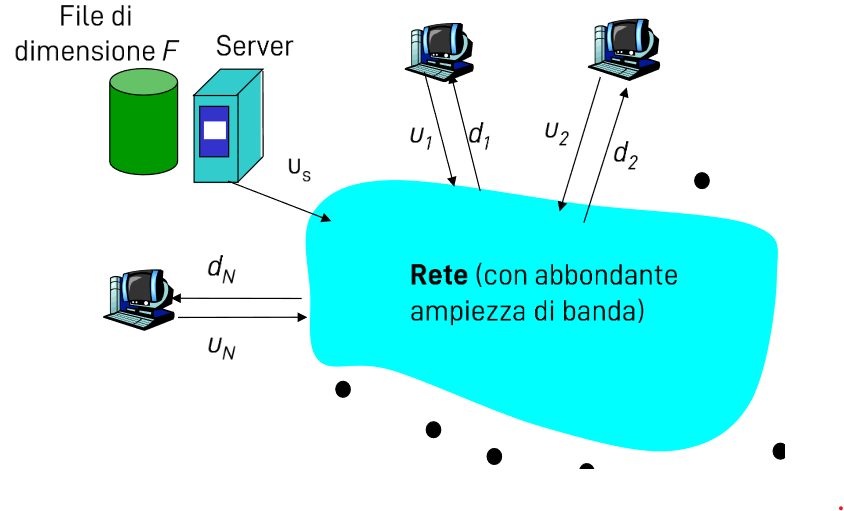
\includegraphics[width=0.5\textwidth]{02/reteP2P.png}
            \caption{Distribuzione di file in modalità \texttt{P2P}}
        \end{figure}
        \paragraph{Domanda:} Tenendo a mente la soprastante figura, ci si può chiedere: Quanto tempo ci vuole per distribuire un file da un server a $ N $ \textit{peer}?\newline
        Consideriamo: \textbf{$U_s$} il \textit{bitrate} in uscita del collegamento di accesso del server, \textbf{$U_i$} bit rate di upload del collegamento di accesso dell \textit{i}-esimo \textit{peer} e \textit{$d_i$} il \textit{bitrate} di download del collegamento di accesso dell \textit{i}-esimo \textit{peer}.
        \paragraph{Soluzione \textit{server-client}} In una architettura \textit{server-client} il tempo di distribuzione è dato dal server che deve inviare $N$ copie moltiplicato per la dimensione del file $F$ il tutto diviso per il \textit{bitrate} in uscita del server $U_s$, quindi in formula: $T=\frac{N\cdot F}{U_s}$. Ora il client $i$-esimo impiega il tempo $F/d_i$ per scaricare il file. Per calcolare il tempo per distribuire il file $F$ su $N$ client è uguale al massimo tra il tempo impiegato dal server per la trasmissione ($U_s$) e dal tempo massimo impiegato da un client per scaricare il file ($d_i$), quindi $d_{cs} = \max\left\{\frac{F}{U_s}, \frac{F}{\min(d_i)}\right\}$. Notare come il tempo di distribuzione aumenta linearmente rispetto al numero di \textit{peer}.
        \paragraph{Soluzione per \textit{P2P}} In una architettura \textit{P2P} per calcolare il tempo di distribuzione dobbiamo prima sapere quanto tempo impiega \textit{server} per inviare la prima copia del file $ T_s = \frac{F}{U_s} $ e poi necessitiamo di sapere quanto tempo impiega l'\textit{i}-esimo client per scaricare il file: $T_i= \frac{F}{d_i} $. Dato che poi il \textit{peer} che ha scaricato il file poi può trasmetterlo a sua volta allora il puù veloce tasso di \textit{upload} è: $U_s+\sum_iU_i $. Il tempo totale è dato dunque dal massimo tra: tempo di invio prima copia, tempo massimo di un peer e il tempo di invio di tutte le copie ($\frac{NF}{U_s\sum_iU_i} $), quindi in modo formulare: $ d_{P2P}=\max\left\{\frac{F}{U_s}, \frac{F}{\min(d_i)}, \frac{NF}{U_S+\sum_iu_i}\right\} $. Notare come il tempo di distribuzione a meno di un tempo costate per l'invio della prima copia si riduce all'aumentare del numero di \textit{peer}.
        \subsubsection{BitTorrnet}
            \paragraph{Introduzione} Nel protocollo di \textit{BitTorrent} si usa la distribuzione di file in modo \texttt{P2P} ma sono presenti dei \textit{server} detti \textit{tracker} che mantengono una lista di \textit{peer} partecipanti alla rete. Un nuovo \textit{peer} che vuole scaricare un file si connette al \textit{tracker} e ottiene la lista che stanno scaricando il file. Il \textit{peer} scarica il file da più \textit{peer} contemporaneamente, andando quindi a costituire una rete \textit{torrent}.
            \paragraph{Caratteristiche} I file vengono divisi in \textit{chunk} da $ 256kB $, quando un peer entra a far parte del torrent non possiede nessun \textit{chunk}, dunque si registra al server \textit{tracker} che gli assegna una lista di \textit{neighbors} ovvero vicini dai quali scaricherà i \textit{chunk} del file, quando un \textit{chunk} è scaricato il \textit{peer} lo condivide con gli altri alimentando l'effetto \textit{tit-for-tat}. Una volta che il file è scaricato nella sua completezza il \textit{peer} può lasciare la rete egoisticamente (\textit{leech}) o contribuire a questa (\textit{seeder})
    \subsection{Ricerca delle informazioni}
        I sistemi di tipo \texttt{P2P} devono in qualche modo fornire un indice della posizione dei \textit{peer} e di in quali di questi si può trovare un particolare file, solitamente questo viene fatto attraverso una \textit{Distributed hash table}.
            \subsubsection{File sharing \textit{e-mule}}
                In un sistema come \textit{e-mule} l'indice tiene traccia dinamicamente della posizione dei file che i \textit{peer} condividono, questi condividono i file disponibili. Un nuovo \textit{peer} cerca nell'indice quello che vuole trovare e poi stabilisce una connessione diretta al \textit{peer} contenete il file cercato.
            \subsubsection{Messaggistica istantanea}
                Nel caso della messaggistica istantanea l'indice crea una corrispondenza tra utenti e posizione (ip), quando un utente si registra all'applicazione informa il server della sua posizione, per inviare un messaggio ad un utente il \textit{peer} chiede al server la posizione dell'utente e poi stabilisce una connessione diretta.
            \subsubsection{Directory centralizzata}
                Nel caso di \textit{napster} invece quando un \textit{peer} si connette alla rete informa il server centrale del suo indirizzo ip e del contenuto condiviso, se un altro \textit{peer} cerca il contenuto dal server centrale allora questo restituisce l'indirizzo ip del \textit{peer} che condivide il file e il \textit{peer} può scaricare il file direttamente.
                \paragraph{Problemi} In primo luogo questa \textit{directory centralizzata} costituisce un \textit{Single point of failure}, inoltre essendo un solo punto questo è un importante \textit{bottleneck} infine se vengono condivisi file protetti da \textit{copyright} il server centrale ne è responsabile.
            \subsubsection{\textit{Query flooding}}
                Un sistema che adotta il \textit{query flooding} è completamente distribuito senza un server centrale, ogni \textit{peer} mantiene un indice locale dei file condivisi e quando un \textit{peer} cerca un file invia una \textit{query} a tutti i \textit{peer} vicini che se non hanno il file cercato inoltrano la \textit{query} ai loro vicini e così via. Questo sistema è molto efficiente ma può generare un grande traffico di rete. Una volta trovato il file viene istituita una connessione diretta \texttt{TCP} tra i due \textit{peer}. Questo sistema è molto efficiente ma può generare un grande traffico di rete ed è soggetto ad attacchi di tipo \textit{DoS}, se viene richiesto un file inesistente la \textit{query} viene inoltrata a tutti i \textit{peer} della rete.
\section{Cloud Computing}
    \paragraph{Introduzione} Il \textit{cloud computing} prevede che uno o più \textit{server} reali, organizzati in una architettura ad alta affidabilità e fisicamente collocati in un \textit{data center} del fornitore del servizio. Il fornitore espone delle interfacce per elencare e gestire i propri servizi, un utente amministratore usa queste selezionando i servizi richiesti per accedervi o amministrarlo, infine un utente finale può accedere ai servizi tramite un'interfaccia web o un'applicazione.
    \paragraph{Criticità}
        \begin{itemize}
            \item \textbf{Privacy \& Sicurezza} - I dati sono memorizzati in un server remoto
            \item \textbf{Continuità del servizio} - I servizi sono soggetti a interruzioni e necessitano di connessione internet
            \item \textbf{Problemi internazionali di natura economico-politica} - I dati possono essere soggetti a leggi di paesi diversi
            \item \textbf{Difficoltà di migrazione} - I dati possono essere difficili da migrare una volta che sono stati caricati
        \end{itemize}
    \subsection{\textit{Content Delivery Network} - \texttt{CDN}}
        \paragraph{Introduzione} Una \textit{CDN} è un sistema di server distribuiti che lavorano insieme per fornire contenuti web ad utenti finali con prestazioni elevate e alta affidabilità. Una \textit{CDN} è composta da \textit{server} detti \textit{edge server} che sono distribuiti in tutto il mondo, un \textit{server} centrale detto \textit{origin server} che contiene i contenuti originali e un \textit{server} detto \textit{DNS server}
        \paragraph{Esempio} 
            \begin{itemize}
                \item Un utente richiede un oggetto
                \item Il \textit{DNS server} determina il \textit{edge server CDN} più vicino all'utente
                \item Il \textit{edge server} richiede l'oggetto all'\textit{origin server} e lo memorizza
                \item Il \textit{edge server} invia l'oggetto all'utente
                \item Il \textit{edge server} memorizza l'oggetto per un certo periodo di tempo
                \item Se un altro utente richiede lo stesso oggetto il \textit{edge server} lo invia direttamente
                \item Se l'oggetto non è più richiesto il \textit{edge server} lo elimina
                \item Se l'oggetto cambia il \textit{edge server} lo richiede all'\textit{origin server}
            \end{itemize}
    
    \paragraph{Conclusione} "There is no cloud, it's just someone else's computer"
    \chapter{Il Livello di Trasporto}
\thispagestyle{chapterInit}
\paragraph{Obbiettivi}
    \begin{itemize}
        \item Capire i principi che sono alla base dei servizi di livello di trasporto:
            \subitem Multiplexing/de-multiplexing
            \subitem Trasferimento dati affidabile
            \subitem Controllo di flusso
            \subitem Controllo di congestione
        \item Descrivere i protocolli del livello di trasporto di Internet:
            \subitem TCP: Trasposto orientato alla connessione
            \subitem Controllo di congestione TCP
            \subitem UDP: Trasporto non orientato alla connessione
    \end{itemize}
\section{Servizi a livello di trasporto}
    \paragraph{Introduzione} I \textbf{protocolli di trasporto} forniscono la comunicazione logica tra processi applicativi di host diversi. I protocolli di trasporto vengono eseguiti negli host "terminali" ovvero quelli che generano o consumano i dati. Dal lato di inviante il protocollo di trasporto divide in diversi segmenti i dati ricevuti dal livello di applicazione e li invia al livello di rete. Dal lato di ricevente il protocollo di trasporto riassembla i segmenti ricevuti e li invia al livello di applicazione.
    \paragraph{TCP} Il \textbf{TCP} (Transmission Control Protocol) è un protocollo di trasporto orientato alla connessione. Il TCP fornisce un trasferimento affidabile dei dati, controllo di flusso e controllo di congestione.
    \paragraph{UDP} L'\textbf{UDP} (User Datagram Protocol) è un protocollo di trasporto non orientato alla connessione. L'UDP non fornisce trasferimento affidabile dei dati, controllo di flusso e controllo di congestione.
    \paragraph{Servizi non disponibili} Al momento in internet non è disponibile un servizio di garanzia su ritardi (latenza), e non è disponibile un servizio di garanzia sulla banda (velocità di trasferimento).
\section{Multiplexing e De-multiplexing}
    \paragraph{Introduzione} Il \textbf{multiplexing} è il processo di invio di dati da più socket a un'unica connessione, per identificare il socket di destinazione si utilizza un \textbf{port number}. Il \textbf{de-multiplexing} è il processo di invio dei dati ricevuti al socket corretto in base al port number.
    \subsection{De-multiplexing}
        \paragraph{Come funziona} In primo luogo quando l'\textit{host} riceve un segmento IP contenente: IP del mittente, IP del destinatario, protocollo di trasporto, porta di destinazione e porta di sorgente. L'\textit{host} utilizza l'indirizzo IP del destinatario e la porta di destinazione per inviare il segmento al processo corretto.
        \subsubsection{De-multiplexing senza connessione}
            Per eseguire il de-multiplexing senza connessione si crea un socket per ricevere i dati. Il socket è ora associato a una porta ed a un indirizzo IP. Quando l'\textit{host} riceve il segmento \texttt{UDP}, viene controllato che il numero di porta di destinazione sia uguale alla porta del socket. Se il numero di porta non corrisponde il segmento viene scartato. Se invece il numero di porta corrisponde il segmento viene inviato al processo associato al socket.
            \begin{figure}[H]
                \centering
                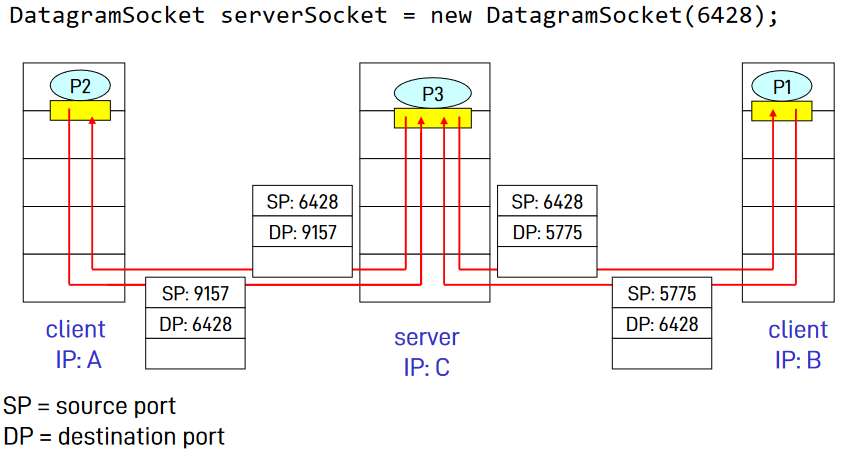
\includegraphics[width=0.5\textwidth]{03/DemultiplexingSenzaConnessione.png}
                \caption{De-multiplexing senza connessione}
            \end{figure}
        \subsubsection{De-multiplexing orientato alla connessione}
            Quando si utilizza un protocollo orientato alla connessione (\texttt{TCP}), il processo di de-multiplexing è leggermente diverso. Il socket infatti è costituito da quattro parametri: indirizzo IP del mittente, indirizzo IP del destinatario, numero di porta di sorgente e numero di porta di destinazione. Quando l'\textit{host} riceve un segmento \texttt{TCP} controlla che i quattro parametri del socket corrispondano ai quattro parametri del segmento. Se i parametri non corrispondono il segmento viene scartato, altrimenti viene inviato al processo associato al socket. Un \textit{host} può supportare più socket contemporaneamente purché cambi almeno uno dei quattro parametri, inoltre i \textit{web server} sono un chiaro esempio di applicazione che utilizza più socket contemporaneamente (su \texttt{HTTP/1.0} un socket per ogni richiesta).\footnote{Se viene allocata una porta ad una connessione, la porta non può essere utilizzata da altre connessioni, quindi nel caso di un \textit{web server} è vero che questo ascolta sulla porta 80, ma quando un client si connette al server, il server apre un socket con una porta dinamica.}
            \begin{figure}[H]
                \centering
                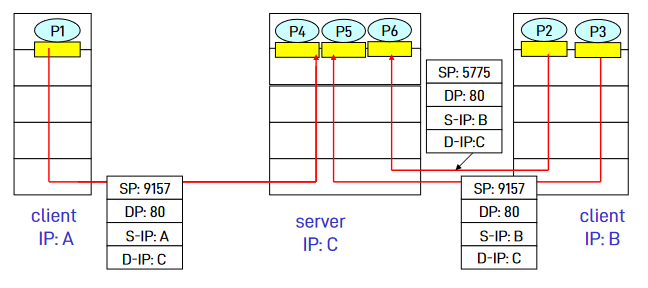
\includegraphics[width=0.5\textwidth]{03/DemultiplexingConConnessione.png}
                \caption{De-multiplexing orientato alla connessione}
            \end{figure}
    \subsection{Porte \texttt{TCP}-\texttt{UDP}}
        La destinazione finale di un segmento non è un host ma un processo. L'interfaccia tra l'applicazione e il livello di trasporto è chiamata \textbf{socket} o \textbf{porta} (nel caso di \texttt{UDP} e \texttt{TCP}). Un \textbf{socket} è un indirizzo IP e un numero di porta. Un \textbf{port number} è un numero a 16 bit che identifica un processo all'interno di un host. Esiste una mappatura biunivoca tra un \textbf{port number} e un processo. I servizi standard utilizzano porte ben note con valori tra 0 e 1023. I processi non-standard e le connessioni in ingresso a un client usano numeri fino a 25535 (16 bit).
        \paragraph{Numeri di porte}
            I numeri di porta si classificano come segue:
            \begin{description}
                \item[Statici] Per i servizi standard, es. HTTP (80), FTP (21), SSH (22), Telnet (23), SMTP (25), POP3 (110), IMAP (143), HTTPS (443), ecc.
                \item[Dinamici] (o "ephemeral") per le connessioni in uscita o per porte allocate dinamicamente, es. client web, client FTP, client SSH, client Telnet, client SMTP, client POP3, client IMAP, client HTTPS, ecc.
            \end{description}
            Inoltre è importante dire che le porte di sorgente e di destinazione non sono le stesse in quanto la porta di sorgente è una porta dinamica assegnata dal sistema operativo.
\section{Trasporto senza connessione: \texttt{UDP}}
    \paragraph{Caratteristiche} L'\textbf{UDP} (User Datagram Protocol) è un protocollo di trasporto senza connessione, offre un servizio \textit{best effort} e non fornisce garanzie di consegna, ordine o duplicazione dei dati. Questo in quanto non ha \textit{handshake} iniziale e non mantiene alcuno stato di connessione. 
    \paragraph{Perché esiste \texttt{UDP}} Non richiede di stabilire una connessione, è semplice e veloce, Header di segmento corti, senza controllo di congestione.
    \subsection{Header}
        \begin{figure}[H]
            \centering
            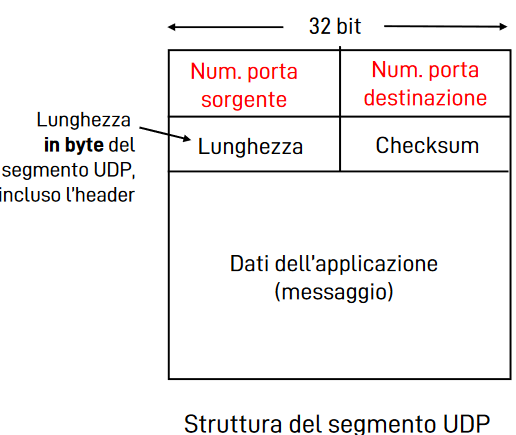
\includegraphics[width=0.3\textwidth]{03/UDPHeader.png}
            \caption{Header di un segmento UDP}
        \end{figure}
        \begin{description}
            \item[Porta di sorgente] Numero di porta del processo mittente.
            \item[Porta di destinazione] Numero di porta del processo destinatario.
            \item[Lunghezza] Lunghezza del segmento in byte.
            \item[Checksum] Utilizzato per rilevare errori nel segmento.
        \end{description}
        \subsubsection{Checksum}
            Il checksum è un campo a 16 bit che viene utilizzato per rilevare errori nel segmento. Questo viene calcolato da entrambe le parti: viene trattato il contenuto come una sequenza di $ 16 $ bit e si sommano tutti i bit (se presente riporto questo viene sommato a sua volta) e viene eseguito il complemento a 1. Il mittente invia il checksum calcolato nel segmento e il ricevente calcola il checksum del segmento ricevuto e lo confronta con il checksum ricevuto. Se i due checksum non corrispondono il segmento viene scartato.
\section[trasferimento dati affidabile]{Principi del trasferimento dati affidabile}
    \subsection{\texttt{ARQ}}
        \textbf{\texttt{ARQ}} o \textit{Automatic Repeat reQuest} è una classe di protocolli che "cercano" di recuperare i segmenti persi o danneggiati. Questa classe usa dei pacchetti speciali per notificare al mittente che un segmento è stato perso o danneggiato. Questi pacchetti speciali sono chiamati \texttt{ACK} (Acknowledgement) e \texttt{NACK} (Negative Acknowledgement).
        \paragraph{Esempi di protocolli basati su \texttt{ARQ}} \begin{itemize}
            \item \textit{Stop-and-Wait}
            \item \textit{Go-Back-N}
            \item \textit{Selective Repeat}
            \item \texttt{TCP}
            \item il protocollo \texttt{MAC} (al livello 2) dei sistemi \texttt{WiFi}
        \end{itemize}
    \subsection{\textit{Stop-and-Wait}}
        Nel protocollo \textit{Stop-and-Wait} il mittente invia una \texttt{PDU} e ne mantiene una copia in memoria, imposta dunque un \textit{timeout} su quel \texttt{PDU}. Attende poi un \texttt{ACK} dal ricevente, se non riceve l'\texttt{ACK} entro il \textit{timeout} invia nuovamente la \texttt{PDU}. Se invece riceve l'\texttt{ACK} controlla che questo non contenga errori, che sia il numero di sequenza corretto e che sia per la \texttt{PDU} inviata. Se tutto è corretto invia la prossima \texttt{PDU}. Il ricevente quando riceve una \texttt{PDU} controlla che il numero di sequenza sia corretto e che la \texttt{PDU} non abbia errori, se tutto è corretto invia un \texttt{ACK} al mittente, de-capsula la \texttt{PDU} ai livelli superiori. Se sono presenti errori nella \texttt{PDU} il ricevente esegue il \textit{drop} della \texttt{PDU}.
        \subsubsection{Efficienza dello \textit{Stop-and-Wait}}
            Assumendo una banda $ R = 1 G-bit/s, 15ms $ di ritardo di propagazione, lunghezza del messaggio $ L = 8000bit $, allora il tempo di trasmissione sarà: $T_{trans} = \frac{L}{R} = \frac{80000}{10^9} = 8\mu s$. Mentre il \textit{throughput} percepito a livello applicativo sarà: $ \frac{L}{T_{trans}+RTT}= \frac{8000}{8\mu s + 30ms} = 33 Kbps $.\footnote{Aggiungiamo della formula il \texttt{RTT} ovvero il \textit{Round Trip Time} che è il tempo che impiega un pacchetto per andare dal mittente al ricevente e ritornare indietro, nel nostro caso lo aggiungiamo per il pacchetto di \texttt{ACK} ed è di $ 30ms $.} Dunque anche se la nostra banda è di $ 1 Gbps $ il \textit{throughput} percepito a livello applicativo è di $ 33 Kbps $, l'efficienza dunque è: $ \frac{T_{trans}}{T_{trans}+RTT} = \frac{0.008}{0.008+30} = 0.00027 $ ovvero $ 0.027\% $.
    \subsection{Protocolli con \textit{pipelining}}
        I protocolli con \textit{pipelining} permettono di inviare più segmenti successivi senza attendere l'\texttt{ACK} del segmento precedente, si allarga dunque il range dei pacchetti di sequenza accettabili. Questo permette di aumentare l'efficienza del trasferimento dati. Esempio di protocolli con \textit{pipelining} sono \textit{Go-Back-N} e \textit{Selective Repeat}.
        \subsubsection{\textit{Throughput} in presenza di \textit{pipelining}}
            Assumiamo la stessa situazione precedente ed un \textit{pipelining} di $ N = 3 $ allora il \textit{throughput} sarà: $ \frac{3L}{T_{trans}+RTT} = \frac{24000}{8\mu s + 30ms} = 100 Kbps $, questo è un miglioramento del $ 300\% $ rispetto allo \textit{Stop-and-Wait}. In generale il \textit{throughput} rispetto al \textit{pipelining} con $ N $ segmenti in parallelo è: $ \frac{N \cdot L}{RTT + T_{trans}} $. Il parametro $ N $ è detto \textit{window size} o "dimensione della finestra".
        \subsubsection{Definizioni}
            \begin{description}
                \item[Finestra di trasmissione $W_T$] Insieme di \texttt{PDU} che il mittente può inviare senza attendere un \texttt{ACK} del ricevente.
                    \subitem Grande al massimo come la memoria allocata dal sistema operativo.
                    \subitem $\left|W_T\right|$ indica la dimensione della finestra.
                \item[Finestra di ricezione $W_R$] Insieme di \texttt{PDU} che il ricevente può ricevere può accettare e memorizzare.
                    \subitem Grande al massimo come la memoria allocata dal sistema operativo.
                \item[Puntatore \textit{low} $W_{LOW}$] Indica il primo segmento della finestra di trasmissione $W_T$.
                \item[Puntatore \textit{high} $W_{HIGH}$] Indica l'ultimo segmento già trasmesso della finestra di trasmissione $W_T$.
            \end{description}
        
        \begin{figure}[H]
            \centering
            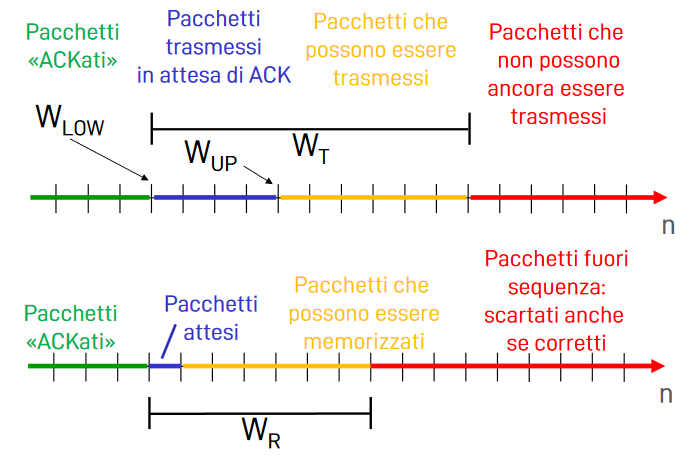
\includegraphics[width=0.5\textwidth]{03/finestrePipelining.png}
            \caption{Finestre di trasmissione e di ricezione}
        \end{figure}
        \subsubsection{\textit{Acknowledgements} - \texttt{ACK}}
            Esistono vari tipi di \texttt{ACK} a seconda del protocollo utilizzato, abbiamo dunque:
            \begin{itemize}
                \item \texttt{ACK} individuale il cui compito è quello di indicare la corretta ricezione di uno specifico pacchetto - \texttt{ACK($n$)} vuol dire ho ricevuto il pacchetto $n$.
                \item \texttt{ACK} cumulativo il cui compito è quello di indicare la corretta ricezione di tutti i pacchetti fino a quello specificato - \texttt{ACK($n$)} vuol dire ho ricevuto tutti i pacchetti fino a $n$ (escluso), mi aspetto il pacchetto $n$.
                \item \texttt{ACK} negativo o \texttt{NACK} il cui compito è quello di indicare la mancata ricezione di un pacchetto - \texttt{NACK($n$)} vuol dire non ho ricevuto il pacchetto $n$, invialo nuovamente.
                \item Esiste poi la tecnica del "\textbf{Piggybacking}", ovvero l'inserimento dell'\texttt{ACK} (di un pacchetto precedente) all'interno di un pacchetto dati successivo.
            \end{itemize}
        \subsubsection{\textit{Go-Back-N}}
            Quando si sceglie di usare il protocollo del tipo \textit{Go-Back-N} questo consiste in: il mittente invia fino ad un numero $ n $ di pacchetti senza aver ricevuto prima \texttt{ACK}, quando un pacchetto è stato ricevuto correttamente viene inviato un \texttt{ACK} cumulativo, se un pacchetto non è stato ricevuto allora i pacchetti successivi vengono scartati in attesa del pacchetto mancante. Dopo un periodo di \textit{timeout} il mittente invia nuovamente tutti i pacchetti a partire dal pacchetto mancante, basandosi sull'ultimo \texttt{ACK} ricevuto. La finestra di trasmissione $ W_T $ è dunque composta da $ n $ pacchetti e non viene spostata finché non si riceve un \texttt{ACK} cumulativo, mentre la finestra di ricezione $ W_R $ è composta da un solo pacchetto.
        \subsubsection{\textit{Selective Repeat}}
            Nel paradigma del \textit{selective repeat} vengono usati \texttt{ACK} singoli, inoltre è presente una finestra di ricezione $ W_R $ composta da $ m $ pacchetti, ciò significa che anche se un pacchetto ricevuto fuori sequenza viene ricevuto allora questo viene comunque "salvato" all'interno di un buffer in attesa del pacchetto nell'ordine corretto. Anche il mittente in caso di \texttt{ACK} fuori sequenza conserva in memoria questo dato e non lo scarta. Quello che succede se un pacchetto non viene ricevuto ma qualche pacchetto (fino a $m-1$) successivo viene ricevuto correttamente è che il mittente invia nuovamente solo il pacchetto mancante, mentre i pacchetti successivi, se sono già stati \texttt{ACK'ati}, non vengono inviati nuovamente e la trasmissione riprende dal primo pacchetto non \texttt{ACK' ato}.
        \paragraph{Spazio dei numeri di sequenza}
            Solitamente se si hanno $ k $ bit a disposizione allora si usa un periodo pari a $ 2^k $, ovvero il periodo massimo con quello spazio di bit. Le finestre di trasmissione per non avere conflitti devono avere somma inferiore al periodo, quindi $ |W_T| + |W_R| < 2^k $.
\section[Trasporto Orientato Connessione \texttt{TCP}]{Trasporto orientato alla connessione \texttt{TCP}}
    \paragraph{\texttt{TCP} - vari standard \texttt{RFC}} Il \texttt{TCP} o \textit{Transmission Control Protocol} è un protocollo di trasporto orientato alla connessione, è stato standardizzato nel \texttt{RFC 793} e successivamente aggiornato con il \texttt{RFC 1122}, \texttt{RFC 1323}, \texttt{2018}, \texttt{2581} ed è in continuo aggiornamento. Questo prevede una connessione \underline{punto-punto} tra mittente e destinatario, è presente un flusso di byte affidabile e consegnato in ordine senza limiti, è presente un meccanismo di \textit{pipelining} e di controllo di congestione per non sovraccaricare la rete. La connessione inoltre (anche se a livelli inferiori non lo è) è \textit{\underline{full-duplex}} ovvero entrambi i lati possono inviare e ricevere dati contemporaneamente. Inoltre il \texttt{TCP} è un protocollo \textit{\underline{stateful}} ovvero mantiene uno stato della connessione, infatti si dice che è orientato alla connessione. Infine ha presente un flusso controllato, il trasmettitore non può inviare dati se il ricevente non è pronto a riceverli.\newpage
    \subsection{Struttura di un pacchetto \texttt{TCP}}
        \begin{figure}[H]
            \centering
            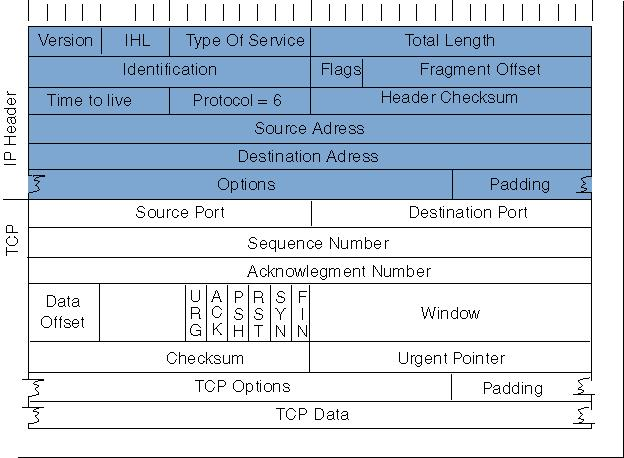
\includegraphics[width=0.45\textwidth]{03/pacchettoTCP.jpg}
            \caption{Struttura di un pacchetto \texttt{TCP}} 
            \footnote{Immagine tratta da \href{https://commons.wikimedia.org/wiki/File:Ntwk_tcp_header.jpg}{Wikimedia Commons} di Gopalpaliwal at English Wikibooks il file è rilasciato sotto licenza Creative Commons \href{https://creativecommons.org/licenses/by-sa/3.0/deed.en}{Attribution-Share Alike 3.0 Unported}.}
        \end{figure}
        Nel pacchetto \texttt{TCP} sono presenti i seguenti campi principali:
        \begin{description}
            \item[Source Port] Porta di sorgente.
            \item[Destination Port] Porta di destinazione.
            \item[Sequence Number] Numero di sequenza del primo byte del segmento.
            \item[Acknowledgement Number] Numero di sequenza del prossimo byte atteso.
            \item[Data Offset] Lunghezza dell'header in parole di 32 bit.
            \item[URG] Flag che indica la presenza di dati urgenti.
            \item[ACK] Flag che indica la presenza di un campo \texttt{ACK}.
            \item[PSH] Flag che indica che i dati devono essere passati al livello superiore.
            \item[PST] Flag che indica l'inizio di una connessione.
            \item[SYN] Flag che indica la sincronizzazione dei numeri di sequenza.
            \item[FIN] Flag che indica la chiusura della connessione.
            \item[Window] Dimensione della finestra di ricezione. (RWND)
            \item[Checksum] Utilizzato per rilevare errori nel segmento (contiene oltre ai parametri \texttt{TCP} anche i parametri \texttt{IP} come l'indirizzo IP del mittente e del destinatario, la lunghezza del segmento, il protocollo di trasporto, ecc.).
            \item[Urgent Pointer] Puntatore ai dati urgenti.
            \item[TCP Options] Opzioni aggiuntive. (opzionali)
            \item[Padding] Padding per allineare il segmento a 32 bit.
            \item[Data] Dati del segmento.
        \end{description}
        \paragraph{Finestra di ricezione (RWND)} La finestra di ricezione è un campo a 16 bit che indica la dimensione della finestra di ricezione del ricevente. Questo campo è utilizzato per il controllo di flusso, infatti il mittente non può inviare dati se la finestra di ricezione del ricevente è piena. La finestra di ricezione è un campo a 16 bit, quindi la dimensione massima della finestra di ricezione è di $ 2^{16} - 1 = 65535 $ byte. In base alla velocità della banda questo campo può essere modificato per evitare che il mittente non sfrutti tutta la banda disponibile.
        \paragraph{Numeri di sequenza \texttt{ACK} di \texttt{TCP}} I numeri di sequenza di \texttt{TCP} sono a 32 bit, questo significa che il numero di sequenza può variare tra $ 0 $ e $ 2^{32} - 1 = 4294967295 $. Il numero di sequenza nella direzione mittente-ricevente può essere diverso da quello nella direzione ricevente-mittente, questo perché i numeri di sequenza sono indipendenti nelle due direzioni, inoltre non è detto che i numeri di sequenza inizino da $ 0 $, infatti possono iniziano solitamente da un numero casuale. Durante la trasmissione di un pacchetto mittente-ricevente può essere allegato anche un campo \texttt{ACK} per la conferma della ricezione del pacchetto precedente tra ricevente-mittente (stessa cosa per la direzione opposta).
        \subsubsection{Lunghezza massima segmento \texttt{MSS} e \texttt{MTU}}
            In quanto il \texttt{TCP} lavora per byte cerca sempre di non inviare un singolo byte solo in quanto sarebbe uno spreco di risorse e di banda. Allo stesso tempo non si può inviare un segmento troppo grande in quanto potrebbe essere frammentato a livello di rete. Viene dunque introdotta una "lunghezza massima" detta \texttt{MSS} (\textit{Maximum Segment Size}) che indica la lunghezza massima di un segmento \texttt{TCP}. La \texttt{MSS} è calcolata come la \texttt{MTU} (\textit{Maximum Transmission Unit}) che è la lunghezza massima di un pacchetto che può essere inviato su una rete a livello di collegamento. A sua volta la \texttt{MTU} viene calcolata da passati al livello \textit{data-link} e può variare da rete a rete. La \texttt{MSS} si riferisce non alla lunghezza di tutto il segmento \texttt{TCP} ma solo al \textit{payload}, ovvero il campo dati del segmento \texttt{TCP}.
            \paragraph{Come si sceglie \texttt{MSS}?} Non esistono meccanismi per comunicarlo, viene dunque adottato un modello del tipo \textit{trial\& error}, ovvero il mittente invia un segmento con una \texttt{MSS} di dimensione $ X $ se si nota che i livelli inferiori sopportano la dimensione $ X $ allora si aumenta la dimensione della \texttt{MSS}, altrimenti se si nota che qualche messaggio inizia ad essere perso si riduce la dimensione della \texttt{MSS}.
                \subparagraph{Valodi di default}: \begin{itemize}
                    \item \texttt{MTU} di ethernet: $ 1500 $ byte (payload inseribile al livello 2)
                    \item Header \texttt{IP}: $ 20 $ byte
                    \item Header \texttt{TCP}: $ 20 $ byte
                    \item \texttt{MSS} di default: $ 1460 $ byte
                \end{itemize}
                \subparagraph{"\textit{Least maximum}"} La più piccola \texttt{MTU} impostabile per \texttt{IP} è di $ 576 $ byte, questo dunque la \texttt{MSS} di minima impostabile è di $ 536 $ byte.
    \subsection{Setup della connessione \texttt{TCP} - \textit{handshake}}
        La procedura di apertura di una connessione \texttt{TCP} è detta \textit{three-way handshake}, questa procedura è composta dai seguenti passaggi:
        \begin{enumerate}
            \item \textbf{Host A} invia un segmento \texttt{TCP} con il flag \texttt{SYN} impostato a \texttt{1} e la porta di sorgente $ A $ e la porta di destinazione $ B $.
            \item \textbf{Host B} riceve il segmento \texttt{TCP} e invia un segmento \texttt{TCP} con il flag \texttt{SYN} impostato a \texttt{1} e il flag \texttt{ACK} impostato a \texttt{1} (avvenuta la ricezione del segmento di \texttt{SYN}) e la porta di sorgente $ B $ e la porta di destinazione $ A $.
            \item \textbf{Host A} riceve il segmento \texttt{TCP} e invia un segmento \texttt{TCP} con il flag \texttt{ACK} impostato a \texttt{1} (avvenuta la ricezione del segmento di \texttt{SYN}) e la porta di sorgente $ A $ e la porta di destinazione $ B $.
        \end{enumerate}
        In tutti questi passaggi il numero di \texttt{ACK} non si riferisce al numero di sequenza del segmento ricevuto ma al numero di sequenza del prossimo segmento atteso. Questo \textit{handshake} è necessario per sincronizzare i numeri di sequenza tra mittente e ricevente.
    \subsection{Chiusura della connessione \texttt{TCP}}
        La procedura di chiusura di una connessione \texttt{TCP} è detta \textit{tearDown}, questa richiede che la connessione sia chiusa in tutte e due le direzioni. Esiste una maniera "gentile" per chiudere la connessione che prevede l'invio di un segmento \texttt{TCP} con il flag \texttt{FIN} impostato a \texttt{1}. A questo punto la controparte riceve il segmento \texttt{TCP} e invia un \texttt{ACK} \& \texttt{FIN}, ora la connessione è \textit{half-closed} ovvero la connessione è chiusa in una direzione ma aperta nell'altra. Quando il primo host riceve \texttt{ACK} \& \texttt{FIN}, ora la connessione è chiusa in entrambe le direzioni. Questo meccanismo è necessario per evitare che i segmenti \texttt{TCP} vengano persi durante la trasmissione.
            \paragraph{Chiusura con \texttt{RST}} Se un host invia un segmento \texttt{TCP} con il flag \texttt{RST} (reset) impostato a \texttt{1} allora la connessione viene chiusa immediatamente senza attendere risposta dall'altra parte. Questo meccanismo è utilizzato per chiudere una connessione in modo "brusco" in caso di problemi.
    \subsection{Tempi \texttt{RTT} e \texttt{RTO}}
        Il \texttt{TCP} deve "impostare" un \textit{timeout} per l'invio e per la ricezione dei segmenti, questo \textit{timeout} è detto \texttt{RTO} (\textit{Retransmission TimeOut}), deve essere dunque un valore superiore al \texttt{RTT} (\textit{Round Trip Time}) ovvero il tempo che impiega un pacchetto per andare dal mittente al ricevente e ritornare indietro. Il \texttt{RTT} può variare nel tempo, quindi il \texttt{RTO} deve essere impostato in modo dinamico, se è troppo basso si rischia di inviare prematuramente un segmento, se è troppo alto si rischia di "aspettare" per troppo tempo. Quindi in sostanza và prima stimato il \texttt{RTT} e poi impostato il \texttt{RTO}, stimiamo il \texttt{RTT} tramite un \textit{sampleRTT} ovvero il tempo tra l'invio del pacchetto e la ricezione dell'\texttt{ACK}. Per mantenere il tempo aggiornato ma non troppo sensibile ai "picchi" che si possono verificare sulla rete viene utilizzata la seguente formula:
        \[ \text{EstimatedRTT} = (1-\alpha) \cdot \text{EstimatedRTT} + \alpha \cdot \text{SampleRTT} \]
        Dove $ \alpha $ è un parametro che indica la "sensibilità" del tempo, se $ \alpha $ è basso allora il tempo sarà poco sensibile ai picchi, se $ \alpha $ è alto allora il tempo sarà molto sensibile ai picchi, questa è una media mobile esponenziale ponderata. Solitamente $ \alpha = 0.125 $.\newline
        Per impostare \texttt{RTO} non ci avvaliamo solamente di questo dato appena ricavato ma anche della deviazione standard del \texttt{RTT} ovvero $$ 
        \text{DevRTT} = (1-\beta) \cdot \text{DevRTT} + \beta \cdot \left| \text{SampleRTT} - \text{EstimatedRTT} \right| $$
        Dove $ \beta $ è un parametro che indica la "sensibilità" della deviazione standard, se $ \beta $ è basso allora la deviazione standard sarà poco sensibile ai picchi, se $ \beta $ è alto allora la deviazione standard sarà molto sensibile ai picchi, questa è una media mobile esponenziale ponderata. Solitamente $ \beta = 0.25 $.\newline
        Infine il \texttt{RTO} viene calcolato come: $$ \text{RTO} = \text{EstimatedRTT} + 4 \cdot \text{DevRTT}\footnote{4 è una costante alla quale tutto il mondo si è accordato ed è usato come misura di sicurezza.} $$
    \subsection{Controllo di flusso \texttt{RWND}}
        Il \texttt{TCP} implementa un meccanismo di controllo di flusso per evitare che il mittente invii troppi dati al ricevente, questo meccanismo è basato sulla finestra di ricezione $ W_R $, il mittente non può inviare dati se la finestra di ricezione del ricevente è piena. La finestra di ricezione è un campo a 16 bit, quindi la dimensione massima della finestra di ricezione è di $ 2^{16} - 1 = 65535 $ byte. Il mittente invia dati fino a $ \min(W_T, W_R) $, dove $ W_T $ è la finestra di trasmissione del mittente e $ W_R $ è la finestra di ricezione del ricevente. Il ricevente invia un segmento \texttt{TCP} con il campo \texttt{Window} impostato alla dimensione della finestra di ricezione, il mittente legge questo campo e regola la dimensione della finestra di trasmissione in base a questo valore.
\section{Principi di controllo di congestione}
    Informalmente la congestione si può tradurre come "troppi trasmettitori stanno mandando troppi dati e la \underline{\textbf{rete}} non riesce a gestirli". Quindi il problema è nella rete e non nel ricevitore. Questo problema si può verificare come: pacchetti persi (\textit{buffer overflow}) o ritardi (\textit{queueing delay}). Il controllo di congestione è un insieme di tecniche che permettono di evitare che la rete vada in congestione. Il controllo di congestione è un problema molto complesso e non esiste una soluzione al problema, esistono però delle tecniche che permettono di mitigare il problema.
    \subsection{Cause/costi della congestione}
        \subsubsection{Scenario 1}
            Assumiamo di avere due trasmettitori e due ricevitori, un \textit{router} con una coda di dimensione infinita, la capacità del link in uscita è $ R $ e non possono esserci ritrasmissioni, allora il \textit{throughput} massimo per ogni trasmettitore è $ R/2 $, ma se entrambi i trasmettitori inviano dati contemporaneamente allora il ritardo salirà asintoticamente con l'avvicinarsi a $ R/2 $.
        \subsubsection{Scenario 2}
            Assumiamo di avere due trasmettitori e due ricevitori, un \textit{router} con una coda di dimensione finita, la capacità del link in uscita è $ R $ e il mittente ritrasmette i pacchetti in timeout, allora considerando il tasso di arrivo dall'applicazione del mittente $\lambda_{in}$ e il tasso percepito dal destinatario $\lambda_{out}$ e il fatto che il mittente invii dati solo quando il router ha spazio nel buffer allora ci troveremmo nel caso ideale ed abbiamo a disposizione un \textit{throughput} di $ R/2 $ per ogni trasmettitore. Se invece il mittente invia dati senza preoccuparsi dello stato del router invia e re-invia i pacchetti in caso di timeout allora per un input di $\lambda_{in}$ pari a $ R/2 $ il \textit{throughput} in uscita sarà di $ R/4 $ (per via delle ritrasmissioni).
\section{Controllo di congestione \texttt{TCP}}
    \paragraph{Alcune cose da dire} Innanzitutto bisogna dire che non esiste un solo algoritmo per il controllo di congestione, esistono infatti molte varianti, ognuna di queste è stata introdotta per rimuovere delle limitazioni della versione precedente. Inoltre l'implementazione di un algoritmo o di un altro dipende spesso dal sistema operativo. Tutte le implementazioni di \texttt{TCP} ragionano in \textit{byte}.
    \paragraph{Caratteristiche} Il controllo di congestione \textbf{adatta il tasso di trasmissione} sulla base delle condizioni della rete, inoltre lo scopo è quello di evitare di \textbf{saturare} e \textbf{congestionare} la rete. 
    \paragraph{Approcci possibili} Esistono due approcci possibili per il controllo di congestione: \begin{itemize}
        \item \textbf{Controllo di congestione \textit{end-to-end}} 
            \subitem Non coinvolge la rete
            \subitem Si capisce se c'è congestione osservando perdite di pacchetti o ritardi
            \subitem Metodo usato da \texttt{TCP}
        \item \textbf{Controllo di congestione assistito dalla rete}
            \subitem I router forniscono feedback ai trasmettitori
            \subitem Un singolo bit per indicare la congestione
    \end{itemize}
    \subsection{\texttt{TCP} \textit{congestion control: additive increase multiplicative decrease} (\texttt{AIMD})}
        \subsubsection{Approccio}
            Il mittente aumenta il tasso di trasmissione cercando di occupare la banda disponibile e diminuisce il tasso di trasmissione quando rileva una perdita. Questo algoritmo segue due passi fondamentali: \begin{itemize}
                \item \textbf{Additive Increase} Aumenta il tasso di trasmissione di 1 \texttt{MSS} ogni \texttt{RTT} finché non si rileva una perdita.
                \item \textbf{Multiplicative Decrease} riduce la finestra (tipicamente di un fattore $ \frac{1}{2} $) quando si rileva una perdita.
            \end{itemize}
        \subsubsection{Perché usare \texttt{AIMD}}
            Per ottenere un \textit{fairness} tra i trasmettitori, infatti se $ k $ sessioni \texttt{TCP} si dividono uno stesso \textit{link} ed è presente un \textit{bottleneck} allora la banda percepita da ogni trasmettitore sarà di $ \frac{R}{k} $.\newline
            Due sessioni in competizione sullo stesso \textit{link} di banda $ R $ allora poniamo un grafico sul quale l'asse delle ascisse è la banda percepita della sessione 1 e l'asse delle ordinate è la banda percepita della sessione 2. 
            \begin{figure}[H]
                \centering
                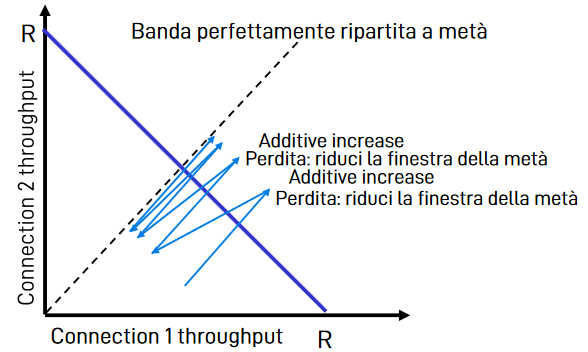
\includegraphics[width=0.5\textwidth]{03/congestione1.png}
                \caption{Grafico di congestione}
            \end{figure}
            Dal grafico si vede come nel tempo le connessioni oscillano verso il punto di intersezione, questo è dovuto al fatto che entrambe le connessioni aumentano la loro banda fino a che non si satura il link, a quel punto entrambe rilevano una perdita e riducono la loro banda dello stesso fattore, questo porta ad un \textit{fairness} tra le due connessioni.
    \subsection{Meccanismi per il controllo di congestione}
        Il controllo di congestione gestisce l'adattamento della cosiddetta finestra di congestione ($CWND$ = numero di byte che il mittente può inviare). \newline
        In \texttt{TCP} ci sono diversi algoritmi per il controllo di congestione, tra i più famosi ci sono: \begin{itemize}
            \item \textbf{In assenza di perdite}
                \subitem Slow Start
                \subitem Congestion Avoidance
            \item Per migliorare l'efficienza di \texttt{TCP} in caso si verifichino perdite
                \subitem Fast Retransmit
                \subitem Fast Recovery
        \end{itemize}
        \textbf{In ogni caso}: $ |W_T| = \min(\texttt{CWND}, \texttt{RWND}) = \min(\texttt{CWND}, |W_R|) $.
        \subsubsection{Slow Start}
            Il \textit{Slow Start} è un algoritmo che prevede che per ogni \texttt{ACK} ricevuto aumento di 1 \texttt{MSS} la finestra di congestione, in questo modo la finestra aumenta esponenzialmente. Questo algoritmo è utilizzato quando la connessione è appena stata aperta e non si conosce la banda disponibile. Il \textit{Slow Start} termina quando la finestra di congestione raggiunge una soglia detta \texttt{SSThresh} (\textit{Slow Start Threshold}) e si passa al \textit{Congestion Avoidance}.
            \paragraph{Algoritmo della fase \textit{slow start}}
            \begin{enumerate}
                \item \textbf{Inizializzazione} \begin{itemize}
                    \item \texttt{CWND} = 1 \texttt{MSS}
                    \item \texttt{SSThresh} = \texttt{RWND} (o \texttt{RWND}/2)
                \end{itemize}
                \item \textbf{\texttt{ACK} valido ricevuto}:\begin{itemize}
                    \item \texttt{CWND} = \texttt{CWND} + 1 \texttt{MSS}
                    \item Sposto $W_{LOW}$ al primo segmento non \texttt{ACK'ato}
                    \item Se \texttt{CWND} $ \geq $ \texttt{SSThresh} allora passo alla fase di \textit{Congestion Avoidance}
                    \item Trasmetto nuovi segmenti (compresi tra $W_{LOW}$ e $W_{HIGH}$)
                \end{itemize}
                \item \textbf{Se scatta un \textit{timeout}}: \begin{itemize}
                    \item Abbasso \texttt{SSThresh} a $\max(\texttt{CWND}/2, 2)$
                    \item Aumento \texttt{RTO} = 2 \texttt{RTO}
                    \item Reimposto \texttt{CWND} = 1 \texttt{MSS}
                    \item Ritrasmetto il segmento in timeout 
                \end{itemize}
            \end{enumerate}
            \subsubsection{Congestion Avoidance}
            Il \textit{Congestion Avoidance} è un algoritmo che prevede che per ogni \texttt{ACK} ricevuto aumento di $ \texttt{MSS}\cdot \frac{\texttt{MSS}}{\texttt{CWND}} $ la finestra di congestione, in questo modo la finestra aumenta linearmente. Quindi per ogni \texttt{RTT} in cui ricevo tutti gli \texttt{ACK} attesi allora aumento di un segmento. Questo algoritmo segue un comportamento lineare e non esponenziale.
            \paragraph{Algoritmo della fase \textit{congestion avoidance}}
            \begin{itemize}
                \item \textbf{Se ricevo un \texttt{ACK} valido}:\begin{itemize}
                        \item \texttt{CWND} = \texttt{CWND} + $ \frac{\texttt{MSS}}{\texttt{CWND}} $ (in byte!)
                        \item Sposto $W_{LOW}$ al primo segmento non \texttt{ACK'ato}
                        \item Trasmetto nuovi segmenti (compresi tra $W_{LOW}$ e $W_{HIGH}$)
                    \end{itemize}
                \item \textbf{Se scatta un \textit{timeout}}: \begin{itemize}
                        \item Passo alla fase di \textit{Slow Start}
                        \item Abbasso $ \texttt{SSThresh} = \max(\texttt{CWND}/2, 2) $
                        \item Aumento \texttt{RTO} = 2 \texttt{RTO}
                        \item Reimposto \texttt{CWND} = 1 \texttt{MSS}
                        \item Ritrasmetto il segmento in timeout
                \end{itemize}
            \end{itemize}
        \subsubsection{Parametri i quali possono essere modificati}
            \begin{itemize}
                \item \textbf{CWND} (\textit{Congestion Window}) Dimensione della finestra di congestione.
                \item \textbf{SSThresh} (\textit{Slow Start Threshold}) Soglia per il \textit{Slow Start}.
                \item \textbf{RTOT} (\textit{Retransmission TimeOut}) Tempo di ritrasmissione.
                \item \textbf{$W_{LOW}\ \&\ W_{HIGH}$} Puntatori alla finestra di trasmissione.
            \end{itemize}
        \subsubsection{\textit{Fast Retransmit}}
            Il \textit{Fast Retransmit} è un algoritmo che prevede che se il mittente riceve tre \texttt{ACK} duplicati allora ritrasmette il segmento richiesto dal \texttt{ACK} duplicato, inoltre il fatto che il mittente riceva tre \texttt{ACK} duplicati indica che c'è una congestione sulla rete si passa dunque alla fase di \textit{Fast Recovery}. Inoltre prendo in considerazione il valore di \texttt{RECOVER}=$W_{UP}$ per determinare quanti segmenti sono stati trasmessi nella rete, in questo modo posso capire quando il processo di \textit{Fast Retransmit} è terminato con successo.
        \subsubsection{\textit{Fast Recovery}}
            Quando ricevo il 3° \texttt{ACK} duplicato entro in \textit{Fast Recovery}, in questa fase avvengono diversi passaggi per evitare di saturare la rete: \begin{itemize}
                \item \textbf{Al 3° \texttt{ACK} duplicato}:\begin{itemize}
                    \item \texttt{SSThresh} = \texttt{CWND}/2
                    \item Supponendo di aver perso solo il segmento in questione: \texttt{CWND} = \texttt{SSthresh} + 3 \texttt{MSS}
                    \item Non sposto $W_{LOW}$
                \end{itemize}
                \item \textbf{Se arrivano altri \texttt{ACK} duplicati allora}: \begin{itemize}
                    \item \texttt{CWND} = \texttt{CWND} +1 \texttt{MSS}
                    \item Non sposto $W_{LOW}$
                \end{itemize}
                \item \textbf{Quando arriva un \texttt{ACK} valido} (che comprende \texttt{RECOVER}): \begin{itemize}
                    \item \texttt{CWND} = \texttt{SSthresh}
                    \item Passo alla fase di \textit{Congestion Avoidance}
                    \item Sposto $W_{LOW}$ al primo segmento non \texttt{ACK'ato}
                \end{itemize}
                \item \textbf{Se arriva un \texttt{ACK} che \underline{non} comprende \texttt{RECOVER}}:\begin{itemize}
                    \item Ritrasmetto il primo segmento non \texttt{ACK'ato}
                    \item \texttt{CWND} = \texttt{CWND}-(numero di segmenti senza \texttt{ACK})+1
                    \item Sposto $W_{LOW}$ al primo segmento non \texttt{ACK'ato}
                \end{itemize}
            \end{itemize}
            \begin{figure}[H]
                \centering
                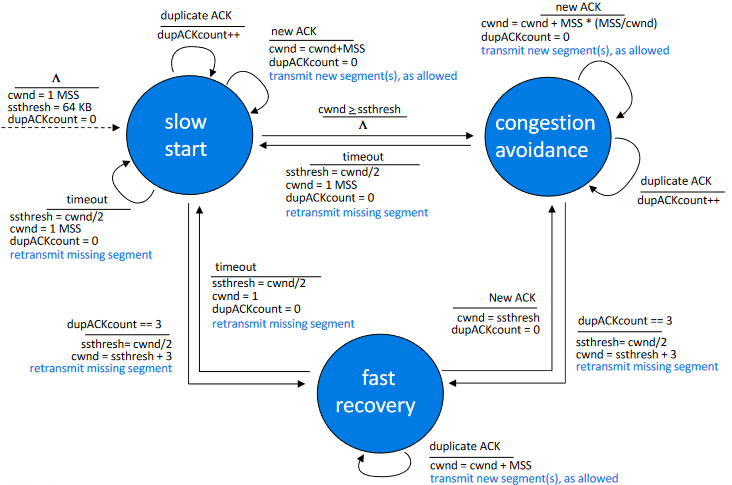
\includegraphics[width=0.4\textwidth]{03/macchinaStatiTCP.png}
                \caption{Macchina a stati di \texttt{TCP}}
            \end{figure}
        \subsubsection{Problemi di equità (\textit{fairness}) in \texttt{TCP}}
            In quanto le applicazione multimediali usano di rado \texttt{TCP} per la trasmissione (ma usano \texttt{UDP}), queste non sono soggette ai controlli di congestione, quindi le connessioni \texttt{TCP} sono penalizzate. Questo avviene in quanto le connessioni \texttt{UDP} trasmettono a velocità costante indipendentemente da fattori esterni.\newline
            Se invece abbiamo due \textit{host} che usano \texttt{TCP} e uno apre (ad es.) $ 9 $ connessioni mentre l'altro ne apre $ 1 $ allora il primo avrà un \textit{throughput} di $ \frac{R}2 $ mentre il secondo avrà un \textit{throughput} di $ \frac{R} {10} $.
    \subsection{Altri algoritmi più recenti per il controllo di congestione}
        Negli algoritmi visti fino ad ora il processo di "rallentamento" della trasmissione avveniva solo in caso di perdita di pacchetti, questo però permette di regolare la banda solo quando è troppo tardi, in quanto deve avvenire una perdita prima che il mittente si renda conto che c'è una congestione. Per ovviare a questo problema sono stati introdotti nuovi algoritmi che permettono di regolare la banda. Questi algoritmi sono: \begin{itemize}
            \item \texttt{CUBIC}
            \item \texttt{BBR}
            \item \texttt{QUIC}
        \end{itemize}
        \subsubsection{\texttt{CUBIC}}
            L'algoritmo \texttt{CUBIC} fa variare la lunghezza della finestra di congestione secondo una funzione cubica nel tempo, questo ne migliora la scalabilità e la stabilità. Questo algoritmo è stato introdotto nel kernel di \texttt{Linux} a partire dalla versione 2.6.19, mentre in \texttt{Windows} è stato introdotto a partire dal 2017.
            \paragraph{Principi del funzionamento} Per un migliore utilizzo e stabilità della rete \texttt{CUBIC} usa sia sia la parte concava che quella convessa della funzione cubica per regolare la finestra di congestione. 
            $$
                \texttt{CWND}_{cubic}(t) = C(t-K)^3 + \texttt{CWND}_{max}
            $$
            Dove $ C $ è una costante, $ K = \sqrt[3]{\frac{\texttt{CWND}_{max}(1-\beta)}{C}} $ e $ \texttt{CWND}_{max} $ è la dimensione massima della finestra di congestione. Per lo standard \texttt{RFC 8312} $ C = 0.4 $ e $ \beta = 0.7 $, ma dopo che è stata rilevata una congestione allora $ \beta = 0.5 $. Inoltre questo algoritmo è "\texttt{TCP}\textit{-friendly}" ovvero non penalizza i flussi \texttt{TCP} legacy che condividono la stessa rete.
        \subsubsection{\texttt{BBR} - \textit{Bottleneck Bandwidth and Round-trip propagation time}}
            L'algoritmo \texttt{BBR} è un algoritmo di controllo di congestione che cerca di massimizzare il \textit{throughput} e minimizzare il ritardo. Questo algoritmo è stato introdotto da \texttt{Google} nel 2016 e si basa non sul rilevamento di perdite ma su due parametri: \begin{itemize}
                \item \textbf{Bottleneck Bandwidth} La banda disponibile sul \textit{bottleneck}.
                \item \textbf{Round-trip propagation time} Il tempo di propagazione del pacchetto.
            \end{itemize}
            Il funzionamento a grandi linee prevede la trasmissione di pacchetti ad una velocità che non \textit{dovrebbe} saturare la rete. Questo infatti è progettato per ridurre la finestra di congestione prima che si verifichi una perdita, in questo modo si dovrebbe riuscire a limitare ritrasmissioni inutili. Un vantaggio di \texttt{BBR} è quello che solo il \textit{server} lo deve implementare e non anche il \textit{client}. Il concetto usato è quello di \textit{pacing} ovvero inserisco nuovi pacchetti nella \texttt{CWND} solo quando il nodo più lento della rete è pronto a riceverli.
            \paragraph{Migliore produttività} Secondo \textit{Google} \texttt{BBR} con un \textit{link} a $10$ Gbps che invia dati lungo un percorso con \texttt{RTT} di $100$ms con tasso di perdita dell'$1\%$ riesce a raggiungere un \textit{throughput} di $3,3$Mbit/s con \texttt{CUBIC} e di $9100$Mbit/s con \texttt{BBR}. Questo è ideale nel caso di connessioni \texttt{HTTP/2} che sfruttano una singola connessione per trasmettere dati.
            \paragraph{Latenza inferiore} \texttt{BBR} riesce a mantenere una latenza inferiore rispetto a \texttt{CUBIC} in quanto riesce a mantenere la banda costante e non satura la rete. Vari studi (sempre di \textit{Google}) hanno dimostrato che su un collegamento di $10$ Mbps con \texttt{RTT} di $40$ ms ed un \textit{bottleneck} di $1000$ pacchetti la latenza di \texttt{BBR} è di soli $43$ ms contro i $1090$ ms di \texttt{CUBIC}.
        \subsubsection{\texttt{QUIC} - \textit{Quick UDP Internet Connections}}
            \texttt{QUIC} è un protocollo di trasporto sviluppato da \texttt{Google} nel 2012 e si prefissa il raggiungimento di due obbiettivi:\begin{itemize}
                \item Evitare fenomeni di \textit{head-of-line blocking}
                \item Ridurre la latenza di \texttt{TCP}
            \end{itemize}
            \texttt{QUIC} può essere implementato a livello applicazione, oltre che a livello di \textit{kernel}. Lo \textit{use case} di questo dovrebbe essere quello delle connessioni \texttt{HTTP/3}. Il principio di funzionamento di questo è che i pacchetti vengono trasmessi tramite una connessione \texttt{UDP} e non \texttt{TCP}, questo permette di evitare i problemi di \textit{head-of-line blocking} in quanto se un pacchetto viene perso allora non si bloccano tutti i pacchetti successivi. Inoltre \texttt{QUIC} permette di ridurre l'\textit{overhead} di connessione in quando incorpora in se stesso lo scambio delle chiavi (o \textit{handshake}) di \texttt{TLS}.
    \subsection{Conclusioni}
        \subsubsection{Meglio dunque \texttt{TCP} o \texttt{UDP}?}
        La scelta tra \texttt{TCP} e \texttt{UDP} dipende da cosa si vuole fare, se si vuole trasmettere dati in modo affidabile e si vuole evitare di saturare la rete allora si deve usare \texttt{TCP}, se invece si vuole trasmettere dati in modo veloce e non si vuole preoccuparsi di perdite di pacchetti allora si deve usare \texttt{UDP}. Questa scelta però non è così libera come sembra, in quanto se si vuole usare il protocollo \texttt{QUIC} necessitiamo di connessione \texttt{UDP} ma molta della nostra infrastruttura blocca le connessioni di questo tipo in quanto non avviene un controllo di congestione e quindi si rischia di saturare la rete. Google ha provato a mostrare come \texttt{QUIC} sia migliore di \texttt{TCP} cercando di "sbloccare" la rete per questo tipo di connessioni, detto ciò i prodotti della serie \textit{chromium} aprono in contemporanea una connessione \texttt{TCP} e una connessione \texttt{UDP} e scelgono quella che ha il \textit{throughput} migliore. 
        \subsubsection{Cambio di rete}
            Con le connessioni \texttt{TCP} le \textit{socket} vengono identificate dalla quadrupla: (IP M.,IP D., Porta M., Porta D.), se si cambia rete allora si cambia anche l'indirizzo IP e quindi la connessione \texttt{TCP} viene persa. Con \texttt{QUIC} invece la connessione viene mantenuta in quanto la \textit{socket} è identificata da un \texttt{ID} e non dall'indirizzo IP.
    \chapter{Il livello di rete}
\label{cap:livelloRete}
\thispagestyle{chapterInit}
\section{Visione d'insieme}
    \paragraph{Obbiettivo del livello di rete} L'obbiettivo principale del livello di rete è quello di permettere la comunicazione tramite reti diverse attraverso apparecchi detti \textit{router} i quali hanno il compito di inoltrare le informazioni verso la destinazione.
    \paragraph{Funzioni principali} Esistono due funzioni principali del livello di rete: \begin{description}
        \item[Inoltro \textit{forwarding}] Questa è una operazione a livello locale che consiste nel prendere un pacchetto in ingresso e inoltrarlo verso l'uscita corretta.
        \item[Instradamento \textit{routing}] Questa è una operazione a livello globale che consiste nel determinare il percorso migliore per inoltrare un pacchetto verso la destinazione. Per questa operazione si utilizzano degli algoritmi di \textit{routing}.
    \end{description}
    Queste due funzioni sono legate tra loro, ma possono essere isolate. Infatti convenzionalmente distinguiamo con \textit{control plane} la parte del livello di rete che si occupa dell'istradamento e con \textit{data plane} la parte che si occupa dell'inoltro. Questa distinzione è utile per capire come funzionano i router.
    \subparagraph{\textit{Data Pane}} Il \textit{data plane} ha funzione a livello locale ad ogni \textit{router}, questo è il livello che determina \underline{come} inoltrare un \textit{datagram} fornendo la funzione di \textit{forwarding}.
    \subparagraph{\textit{Control Plane}} Il \textit{control plane} ha funzione a livello globale, questo è il livello che determina \underline{dove} inoltrare un \textit{datagram} fornendo la funzione di \textit{routing}.
\section{Come è fatto un router}
    Visto a livello "alto" un router è composto da tre livelli principali: \begin{description}
        \item[Terminazione di linea] Questo è il livello più basso del router, è composto da un'interfaccia di rete che si occupa di ricevere i pacchetti e di inviarli al livello successivo.
        \item[Protocollo di livello \textit{data link}] Questo livello si occupa di ricevere i pacchetti dal livello precedente e di inviarli al livello successivo. Inoltre si occupa di fare il controllo degli errori e di gestire il flusso.
        \item[Inoltro e \textit{buffer}] Questo è il livello che si occupa di inoltrare i pacchetti verso la destinazione. Inoltre si occupa di fare il \textit{buffering} dei pacchetti in caso di congestione.
    \end{description}
    \subsection{Sistemi di commutazione}
        I sistemi di commutazione trasferiscono i pacchetti dalle porte di ingresso all'uscita appropriata. Definiamo come \textbf{tasso di comunicazione} la frequenza alla quale i pacchetti vengono portati dall'ingresso all'uscita (spesso è un multiplo della velocità di comunicazione) 
        \subsubsection{Commutazione a memoria}
            Questo è il metodo più semplice, i pacchetti vengono memorizzati in un buffer comune e poi inoltrati verso l'uscita appropriata. Questo metodo è molto semplice ma ha il problema che la velocità di inoltro è limitata dalla velocità di accesso alla memoria.
        \subsubsection{Commutazione a bus}
            Questo metodo consiste nel collegare le porte di ingresso e di uscita tramite un bus, sempre comune a tutte le porte. Questo metodo risulta lento in quanto non possono essere trasferiti più pacchetti contemporaneamente anche se le porte di ingresso e di uscita sono diverse. Il \texttt{Cisco 5600} è un esempio di router che utilizza questo metodo e riesce a trasferire fino a 32 Gbit/s.
        \subsubsection{Commutazione a matrice}
            Questo metodo consiste nel collegare le porte di ingresso e di uscita tramite una matrice di commutazione. Questo metodo è molto veloce in quanto permette di trasferire più pacchetti contemporaneamente in quanto se le porte sono differenti allora basta attivare i vari collegamenti della matrice. Questo metodo è molto veloce ed ispirato ai primi commutatori telefonici. Il \texttt{Cisco 12000} è un esempio di router che utilizza questo metodo e riesce a trasferire fino a 60 Gbit/s.
    \subsection{Accodamenti}
        Gli accodamenti sono utilizzati per evitare la perdita di pacchetti in caso di congestione dell'apparecchio di rete. Questo è un problema molto comune in quanto i router sono dispositivi molto veloci e le porte di uscita sono molto più lente. Per evitare la perdita di pacchetti si utilizzano delle code che permettono di memorizzare i pacchetti in attesa di essere inoltrati.
        Le code possono essere formate in ingresso, quando una stessa porta di uscita è condivisa da più porte di ingresso e quindi una porta di uscita può essere congestionata. Le code possono essere formate in uscita, quando una porta di uscita ha un \textit{link} più lento rispetto alla velocità di inoltro dei pacchetti tramite le porte di ingresso o il commutatore di pacchetto.
        \paragraph{Quanta memoria serve per i \textit{buffer}} Secondo \texttt{RFC 3439} la quantità di memoria necessaria per i buffer è data dalla formula: \[M = \frac{RTT \cdot C}{\sqrt{N}}\] Dove: \begin{description}
            \item[$M$] è la memoria necessaria per il buffer
            \item[$RTT$] è il tempo di round trip
            \item[$C$] è la capacità del collegamento
            \item[$N$] è il numero di connessioni
        \end{description}
        \paragraph{Meccanismi di \textit{scheduling}}
            I meccanismi di \textit{scheduling} sono utilizzati per decidere quale pacchetto inoltrare quando si ha la possibilità di inoltrare più pacchetti. Il meccanismo più semplice è il \textit{First In First Out} (\texttt{FIFO}) che inoltra i pacchetti in ordine di arrivo. Inoltre viene applicata una politica di scarto dei pacchetti in caso di buffer pieno. Questa politica può essere: \begin{description}
                \item[\textit{Drop Tail}] Questa politica scarta i pacchetti in arrivo quando il buffer è pieno.
                \item[\textit{Random Early Detection}] Questa politica scarta i pacchetti in arrivo in modo casuale quando il buffer è pieno.
                \item[\textit{Priority Drop}] Questa politica scarta i pacchetti in arrivo in base alla priorità.
            \end{description}
            La politica di scarto dei pacchetti dipende dall'implementazione del router.
\section{Il protocollo \texttt{IP}}
    \subsection{Il formato del \textit{datagram} \texttt{IP} (\texttt{IPv4})}
        \begin{figure}[H]
            \centering
            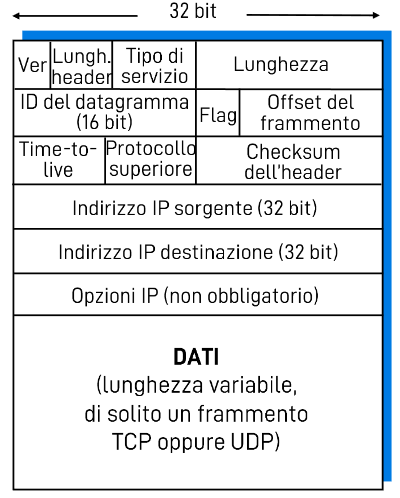
\includegraphics[width=0.36\textwidth]{04/datagramIPv4.png}
            \caption{Il formato del \textit{datagram} \texttt{IP} (\texttt{IPv4})}
            \label{fig:IPv4Header}
        \end{figure}
        Il formato del \textit{datagram} \texttt{IP} è composto da 20 byte di intestazione e da un campo dati. Il campo dati può contenere fino a 65.535 byte.  Di seguito si riportano i vari campi dell'intestazione:
        \begin{description}
            \item[VER] (4 bit) Questo campo contiene la versione del protocollo \texttt{IP} utilizzato.
            \item[Lunghezza \textit{header}] (4 bit) Questo campo contiene la lunghezza dell'intestazione in parole da 32 bit. (=5 se non ci sono opzioni)
            \item[Tipo di servizio - \texttt{ToS}] (8 bit) Questo campo contiene informazioni sul tipo di servizio richiesto.
            \item[Lunghezza totale] (16 bit) Questo campo contiene la lunghezza totale del \textit{datagram} in byte.
            \item[Identificativo] (16 bit) Questo campo contiene un numero univoco per il \textit{datagram}.
            \item[Flag] (3 bit) Questo campo contiene i flag per il frammento. Il primo bit è il bit di \textit{Don't Fragment}, il secondo bit è il bit di \textit{More Fragment} e il terzo bit è il bit di \textit{Fragment Offset}.
            \item[Offset] (13 bit) Questo campo contiene l'offset del frammento. (Espresso in multipli di 8 byte)
            \item[\textit{Time To Live} - \texttt{TTL}] (8 bit) Questo campo contiene il numero di \textit{hop} massimo che il \textit{datagram} può fare.
            \item[Protocollo] (8 bit) Questo campo contiene il protocollo di trasporto che si trova nel campo dati.
            \item[Checksum] (16 bit) Questo campo contiene il checksum dell'intestazione.
            \item[Indirizzo IP sorgente] (32 bit) Questo campo contiene l'indirizzo IP sorgente.
            \item[Indirizzo IP destinazione] (32 bit) Questo campo contiene l'indirizzo IP destinazione.
            \item[Opzioni] (variabile) Questo campo contiene le opzioni del \textit{datagram}.
            \item[Padding] (variabile) Questo campo contiene il padding per allineare l'intestazione a multipli di 32 bit.
        \end{description}
    \subsection{\texttt{MTU} e Frammentazione}
        La \texttt{MTU} (\textit{Maximum Transmission Unit}) è la dimensione massima di un pacchetto che può essere trasmesso su un collegamento, ogni \textit{hardware} specifica il proprio \texttt{MTU}. Se un \textit{datagram} è più grande della \texttt{MTU} allora il \textit{datagram} viene frammentato in pacchetti più piccoli. Questo processo è chiamato \textit{frammentazione}. I pacchetti frammentati vengono poi ricomposti alla destinazione.
        \paragraph{Valori Standard \texttt{MTU}} Per alcuni tipi di collegamenti sono stati definiti dei valori standard di \texttt{MTU}. Ad esempio per le reti Ethernet la \texttt{MTU} è di $1500$ byte, per le reti \texttt{WLAN 802.11} la \texttt{MTU} è di $2304$ byte,\dots. In un collegamento tra due \textit{host} possono essere presenti due valori di \texttt{MTU} diversi
        \subparagraph{Esempio} Supponendo che per raggiungere un host \texttt{B} si debba passare prima da una rete con $1500$ byte di \texttt{MTU} e poi da una rete con $1000$, tutto ciò tramite un router \texttt{R}. Allora quando il \textit{router} \texttt{R} riceve il datagram di $1500$ byte lo frammenta in due pacchetti di $1000$ byte e $500$ byte. I pacchetti vengono quindi inoltrati alla destinazione. Quando l'host \texttt{B} riceve i pacchetti li ricomponi e li passa al livello di trasporto.
        
    \subsection{Indirizzamento e \texttt{NAT}}
        \subsubsection{Indirizzi \texttt{IP}}
            Un indirizzo \texttt{IP} è composto da $32$ bit ed è associato ad un'interfaccia di rete. Una interfaccia è una connessione tramite mezzo fisico o logico, solitamente ogni \textit{host} ha una o più interfacce di rete.
            \paragraph{Caratteristiche indirizzi \texttt{IP}} Gli host e i router devono usare le stesse convenzioni per gli indirizzi \texttt{IP}, inoltre ogni indirizzo \texttt{IP} deve essere unico e raggiungibile da un qualsiasi punto di internet. Quando si invia un pacchetto \texttt{IP} si invia l'indirizzo \texttt{IP} sorgente e l'indirizzo \texttt{IP} destinazione. I \textit{router} sono apparati di rete che quando ricevono un pacchetto \texttt{IP} decidono dove inoltrarlo in base all'indirizzo \texttt{IP} di destinazione.
            \paragraph{Norazione indirizzo \texttt{IP}} Gli indirizzi \texttt{IP} sono composti da $4$ gruppi di $8$ bit e sono scritti in notazione decimale a punti. Ogni gruppo di $8$ bit è espresso in decimale e separato da un punto. Gli indirizzi disponibili vanno dà: $0.0.0.0$ a $255.255.255.255$ 
            \paragraph{Gerarchie indirizzi \texttt{IP}} Gli indirizzi \texttt{IP} sono organizzati in una struttura gerarchica. Inoltre solitamente sono divisi in due parti: \begin{description}
                \item[Parte di rete] Questa parte identifica la rete a cui appartiene l'indirizzo \texttt{IP}.
                \item[Parte di \textit{host}] Questa parte identifica l'\textit{host} all'interno della rete.
            \end{description}
            \subparagraph{Classi di indirizzi \texttt{IP}} Gli indirizzi \texttt{IP} sono divisi in classi sulla base dei primi bit dell'indirizzo e dalla lunghezza del prefisso: \begin{description}
                \item[Classe \texttt{A}] Gli indirizzi di classe \texttt{A} hanno il primo bit a \texttt{0} e sono composti da $8$ bit di rete e $24$ bit di \textit{host}. Gli indirizzi vanno da $0.0.0.0$ a $ 127.255.255.255$ e sono riservati per le reti molto grandi.
                \item[Classe \texttt{B}] Gli indirizzi di classe \texttt{B} hanno i primi due bit a \texttt{10} e sono composti da $16$ bit di rete e $16$ bit di \textit{host}. Gli indirizzi vanno da $128.0.0.0$ a $191.255.255.255$ e sono riservati per le reti di medie dimensioni.
                \item[Classe \texttt{C}] Gli indirizzi di classe \texttt{C} hanno i primi tre bit a \texttt{110} e sono composti da $24$ bit di rete e $8$ bit di \textit{host}. Gli indirizzi vanno da $192.0.0.0$ a $223.255.255.255$ e sono riservati per le reti di piccole dimensioni.
                \item[Classe \texttt{D}] Gli indirizzi di classe \texttt{D} hanno i primi quattro bit a \texttt{1110} e sono riservati per i \textit{multicast}.
                \item[Classe \texttt{E}] Gli indirizzi di classe \texttt{E} hanno i primi quattro bit a \texttt{1111} e sono riservati per usi futuri.
            \end{description}
        \subsubsection{Assegnazione indirizzi \texttt{IP}}
            Gli indirizzi \texttt{IP} sono assegnati dalla \texttt{ICANN} (\textit{Internet Corporation for Assigned Names and Numbers}) che riserva una intera classe ai \texttt{ISP} (\textit{Internet Service Provider}) e poi questi assegnano gli indirizzi ai propri clienti. Gli indirizzi \texttt{IP} sono assegnati in modo gerarchico e quindi un \texttt{ISP} può assegnare un intero blocco di indirizzi ad un altro \texttt{ISP} e questo può assegnare un blocco di indirizzi ad un altro \texttt{ISP} e così via.
    \subsection{Indirizzamento \textit{classless}}
        In quanto ci si è accorti che con la suddivisione degli indirizzi in classi si stava sprecando molti indirizzi, si è deciso di passare ad un indirizzamento \textit{classless}. Questo tipo di indirizzamento permette di avere una suddivisione più flessibile degli indirizzi, in quanto possiamo richiedere al nostro \texttt{ISP} solo un \textit{range} di indirizzi e non una classe intera, ad esempio l'\texttt{ISP} può usare un prefisso di $26$ bit per identificare la rete nel mondo e successivamente usare i restanti $6$ bit per identificare tutti gli \textit{host} della rete.
        In questa situazione se un \texttt{ISP} ha acquistato una rete di classe \texttt{C} e ha bisogno di dividere la rete in quattro clienti allora può dividere la rete in $4$ sotto-reti e assegnare un prefisso di $26$ bit ($24$ per la classe \texttt{C} e $2$ per le sotto-reti) e i restanti $6$ bit per gli \textit{host} di ogni sotto-rete.
        \subsubsection{Maschere di rete}
            In quanto ora non si ha più una suddivisione fissa degli indirizzi, si è deciso di introdurre le \textit{maschere di rete}. Queste maschere sono composte da $32$ bit e sono composte da una parte di $1$ quelli che identificano il prefisso di rete e da una parte di $0$ che identificano gli \textit{host} della rete. Ad esempio la maschera di rete per una rete di classe \texttt{C} è $11111111.11111111.11111111.00000000$.
            \paragraph{Peché si usa?} La maschera di rete viene usata per identificare la rete di appartenenza di un indirizzo IP. Per fare ciò si fa un'operazione di \texttt{AND} tra l'indirizzo IP di destinazione e la maschera di rete. Se il risultato è uguale all'indirizzo di rete allora l'indirizzo IP appartiene alla rete. Quindi se il prefisso di rete è $128.10.0.0$ ovvero: \[10000000.00001010.00000000.00000000\] e la maschera di rete è $255.255.0.0$ ovvero: \[11111111.11111111.00000000.00000000\] e l'indirizzo IP di destinazione di un determinato pacchetto è: $128.10.2.3$ ovvero: \[10000000.00001010.00000010.00000011\] allora facendo l'operazione di \texttt{AND} tra l'indirizzo IP e la maschera di rete si ottiene: \[\begin{aligned}
                10000000.00001010.00000010.00000011 &\\
                11111111.11111111.00000000.00000000 &\\
                \hline
                10000000.00001010.00000000.00000000&=128.10.0.0
            \end{aligned}
            \] Quindi l'indirizzo IP appartiene alla rete e il pacchetto viene inoltrato a quella determinata porta di uscita.
        \subsubsection{Notazioni \texttt{CIDR}}
            \texttt{CIDR} o \textit{Classless Inter-Domain Routing} è un metodo per rappresentare le maschere di rete. Questo metodo consiste nel rappresentare la maschera di rete con un prefisso di bit. Ad esempio la maschera di rete $/24$ è uguale alla maschera di rete $11111111.11111111.11111111.00000000$, ovvero una maschera di rete di classe \texttt{C}, quindi i primi $3$ gruppi di bit sono appartenenti all'\textit{network-id} e l'ultimo gruppo di bit è appartenente all'\textit{host-id}. La notazione prevede inoltre che gli indirizzi \texttt{IP} siano rappresentati nel seguente modo: \texttt{ddd.ddd.ddd.ddd/m} dove ogni singolo \texttt{d} rappresenta un gruppo di bit e \texttt{m} rappresenta il numero di bit del prefisso di rete.
            \paragraph{Esempio} L'indirizzo $193.168.32.199/26$ ha un prefisso di rete di $26$ bit, quindi il \textit{network-id} è: $$11000001.1010100.000000010.11$$ e l'\textit{host-id} è $$00111$$ Esistono dunque $2^6=64$ indirizzi \texttt{IP} nella rete.
            \paragraph{Inoltro con \texttt{CIDR}} L'inoltro con \texttt{CIDR} è molto semplice e non differisce dall'inoltro con le classi. Infatti si fa l'operazione di \texttt{AND} tra l'indirizzo \texttt{IP} di destinazione e la maschera di rete e si confronta il risultato con l'indirizzo di rete. Se il risultato è uguale all'indirizzo di rete allora l'indirizzo \texttt{IP} appartiene alla rete e il pacchetto viene inoltrato alla porta di uscita corretta. Nella situazione in cui ci siano più reti che corrispondono al risultato dell'operazione di \texttt{AND} allora si sceglie la rete con il prefisso più lungo in quanto si presume che questa sia la rete più specifica e quindi la più breve.
            \paragraph{Aggregazione dei percorsi} L'aggregazione dei percorsi è una tecnica che permette di ridurre il numero di percorsi che un router deve memorizzare. Questa tecnica consiste nel raggruppare più reti in un'unica rete più grande. Questa tecnica è molto utile in quanto permette di ridurre il numero di percorsi che un router deve memorizzare e quindi di velocizzare l'inoltro dei pacchetti. Esempio se un \texttt{ISP} controlla tutte le reti $200.23.16.0/23$, $200.23.18.0/23$\dots $200.23.30.0/23$ allora può raggruppare tutte queste reti in un'unica rete $200.23.16.0/20$
            \paragraph{Inoltro di default} L'inoltro di default è una tecnica "\textit{last resource}" usata nel caso in cui non si trovi nessuna corrispondenza tra l'indirizzo \texttt{IP} di destinazione e le reti memorizzate nel router. In questo caso il router inoltra il pacchetto alla porta di uscita di default definita dal router e che solitamente è la porta di uscita verso internet. In questo caso nel router è presente una rotta con \texttt{IP} di destinazione $0.0.0.0$ e maschera di rete $/0$, la cui combinazione è sempre vera per qualunque indirizzo, per la regola del "prefisso più lungo" il router inoltra il pacchetto alla porta di uscita di default solo se non trova nessuna corrispondenza tra l'indirizzo \texttt{IP} di destinazione e le reti memorizzate nel router.
        \subsubsection{Tabella di routing}
            Nella tabella di routing oltre all'associazione "maschera di rete - porta di uscita" è necessario memorizzare anche l'indirizzo \texttt{IP} del prossimo \textit{router} a cui inoltrare il pacchetto, questo in quanto sapere che il pacchetto deve essere inoltrato ad una determinata porta di uscita non è sufficiente se fossero presenti più dispositivi connessi alla stessa porta di uscita.
    \subsection{Tipi di indirizzi}
        In quanto gli indirizzi \texttt{IP} disponibili sono $2^{32}$ e il numero di dispositivi connessi a internet è molto maggiore, si è deciso di introdurre dei tipi di indirizzi pubblici e privati, in modo da risparmiare indirizzi \texttt{IP} pubblici e di proteggere la rete interna da attacchi esterni.
        \subsubsection{Indirizzi pubblici e privati}
            Gli indirizzi \texttt{IP} sono divisi in due categorie: \begin{description}
                \item[Indirizzi pubblici] Gli indirizzi pubblici sono indirizzi che possono essere raggiunti da qualsiasi punto di internet. Questi indirizzi sono assegnati dalla \texttt{ICANN} e sono unici.
                \item[Indirizzi privati] Gli indirizzi privati sono indirizzi che non possono essere raggiunti da internet. Questi indirizzi sono riservati per le reti private e non possono essere usati per comunicare con internet, vengono bloccati dai router. Gli indirizzi privati sono: \begin{itemize}
                    \item Da \texttt{10.0.0.0} a \texttt{10.255.255.255} (\texttt{10.0.0.0/8})
                    \item Da \texttt{172.16.0.0} a \texttt{172.31.255.255} (\texttt{172.16.0.0/12})
                    \item Da \texttt{192.168.0.0} a \texttt{192.168.255.255} (\texttt{192.168.255.255/16})
                \end{itemize}
            \end{description}
        \subsubsection{\textit{Network Area Translation} \texttt{NAT}}
            Il \texttt{NAT} è una tecnica che permette di tradurre gli indirizzi privati in indirizzi pubblici e viceversa. Questo permette ai dispositivi di una rete privata di accedere a internet senza avere un indirizzo \texttt{IP} pubblico. Il \texttt{NAT} è un protocollo appartenente al \textit{router} funzionante nel seguente modo:
            \begin{enumerate}
                \item Il \textit{router} sostituisce l'indirizzo \texttt{IP} di sorgente e la porta di sorgente del pacchetto con il proprio indirizzo \texttt{IP} pubblico e una porta casuale.
                \item Il \textit{router} memorizza l'associazione tra l'indirizzo \texttt{IP} e porta originale con l'indirizzo \texttt{IP} pubblico e la porta generata.
                \item Viene inoltrato il pacchetto alla rete di destinazione, seguendo la tabella di routing.
                \item Quando il pacchetto di risposta arriva al \textit{router}, il \textit{router} sostituisce l'indirizzo \texttt{IP} di destinazione e la porta di destinazione con l'indirizzo \texttt{IP} privato e la porta originale.
                \item Il \textit{router} inoltra il pacchetto alla rete privata.
            \end{enumerate}
            \paragraph{Vantaggi/svantaggi del \texttt{NAT}} In quanto il numero di porta è costituito da $16$ bit, il numero di porte disponibili è $2^{16}=65536$, quindi il \texttt{NAT} permette di avere fino a $65536$ dispositivi connessi alla stessa rete privata. Il "problema" è che il protocollo \texttt{NAT} viola l'architettura a livelli, in quanto dispositivo di rete il \textit{router} non dovrebbe agire sulle porte. La mancanza di \texttt{IP} dovrebbe essere risolta con l'introduzione di \texttt{IPv6} (anche se lentamente). La sola esistenza di \texttt{NAT} deve essere tenuta in considerazione quando si progettano applicazioni (come una rete \texttt{P2P} che non funziona con \texttt{NAT}). Infine se si vuole accedere ad un dispositivo con \texttt{NAT} da internet è necessario usare altri protocolli come \textit{Port Forwarding}, \texttt{UPnP} o altri.
            \subparagraph{\texttt{NAT} può essere utile} Oltre a risparmiare indirizzi \texttt{IP} pubblici, il \texttt{NAT} può essere utile per ovviare a problemi di routing, assumiamo per esempio che un router (al quale non abbiamo accesso) imposti una regola che impedisca l'uscita di pacchetti verso la nostra rete "interna" \texttt{B}, ma permetta che pacchetti verso la rete "pubblica" \texttt{P} vengano inoltrati. In questo caso il \texttt{NAT} può essere utile per far passare i pacchetti dalla rete "interna" \texttt{B} alla rete "interna" \texttt{A} senza modificare le regole di routing. Questo grazie al fatto che il \texttt{NAT} modifica l'indirizzo \texttt{IP} di sorgente, il router non riconosce i pacchetti come provenienti dalla rete "interna" \texttt{A} e quindi li inoltra.
        \subsubsection{Indirizzi \texttt{IP} speciali}
            Gli indirizzi \texttt{IP} speciali sono indirizzi che non possono essere assegnati ad un'interfaccia di rete. Questi indirizzi sono usati per scopi speciali e non possono essere usati per comunicare con internet. Alcuni tipi di indirizzi speciali sono: \begin{itemize}
                \item Indirizzi che identificano tutta la rete
                \item Indirizzi che permettono il \textit{broadcast} a tutti gli \textit{host} della rete
                \item Indirizzi che permettono il \textit{broadcast} in una rete locale (\textit{Limited broadcast address})
                \item Indirizzi di \textit{localhost}
                \item Indirizzi di \textit{loopback}
                \item Indirizzi di \textit{multicast}
                \item Indirizzi di \textit{link-local}
            \end{itemize}
            \paragraph{Identificativi di tutta la rete} Gli indirizzi che identificano tutta la rete sono indirizzi che identificano tutta la rete. Questi indirizzi sono usati per identificare la rete e non possono essere assegnati ad un'interfaccia di rete, questi sono identificati con tutti i bit della parte di \textit{host} a $0$. Ad esempio l'indirizzo \texttt{128.211.0.16/28} identifica tutta la rete
            \paragraph{Indirizzi di \textit{broadcast}} Per il \textit{Directed Broadcast Address} si ha che l'indirizzo di \textit{broadcast} è l'indirizzo che permette di inviare un pacchetto a tutti gli \textit{host} della rete. Questo indirizzo è identificato con tutti i bit della parte di \textit{host} a $1$. Ad esempio l'indirizzo \texttt{128.211.0.31/28} è l'indirizzo di \textit{broadcast} per la rete \texttt{128.211.0.16/28}
            \paragraph{Indirizzi di \textit{broadcast} locale} L'indirizzo di \textit{broadcast} locale è l'indirizzo che permette di inviare un pacchetto a tutti gli \textit{host} della rete locale. Questo indirizzo è identificato con tutti i bit dell'indirizzo a $1$. Quindi l'indirizzo \texttt{255.255.255.255} è l'indirizzo di \textit{broadcast} locale, anche se possa sembrare globale questo rimane locale perché non viene inoltrato alla rete pubblica.
            \paragraph{Indirizzi di \textit{localhost}} Per le regole del protocollo \texttt{TCP/IP} necessitiamo di un indirizzo \texttt{IP} anche per richiedere l'assegnazione di un indirizzo \texttt{IP} allora si è deciso di riservare un indirizzo \texttt{IP} ovvero: \texttt{0.0.0.0} che viene usato solo per le prime comunicazioni all'interno di una rete per "chiedere" l'assegnazione di un indirizzo \texttt{IP}
            \paragraph{Indirizzi di \textit{loopback}} Indirizzo \texttt{IP} riservato per il \textit{loopback} del PC o del dispositivo. Questo indirizzi sono \texttt{127.0.0.0/8}, ma il più comune è \texttt{127.0.0.1}
            \paragraph{Indirizzi di \textit{multicast}} Tutti gli indirizzi \texttt{IP} che iniziano con \texttt{1110} sono indirizzi di \textit{multicast}, molti apparati di rete bloccano il traffico di \textit{multicast} per evitare attacchi.
            \paragraph{Indirizzi \texttt{IP} \textit{local}} Sono indirizzi che non vengono assegnati pubblici ma vengono assegnati autonomamente se ci si aspettava che l'indirizzo \texttt{IP} venisse assegnato da un apparato esterno ma ciò non è avvenuto. Questi indirizzi sono appartenenti alla rete $194.254.0.0/16$ 
            \paragraph{Indirizzi \texttt{IP} dei \textit{router}} Un \textit{router} per definizione ha almeno $2$ interfacce di rete, quindi ha almeno $2$ indirizzi \texttt{IP}. Questo non limita un \textit{router} ad avere solo $1$ indirizzo \texttt{IP} per ogni interfaccia di rete. Da ricordare che un indirizzo \texttt{IP} non è associato ad un \textit{host} ma ad un'interfaccia di rete su un \textit{host}. La molteplicità di indirizzi \texttt{IP} per una sola interfaccia di rete risulta utile se ad esempio volgiamo suddividere la rete interna in più reti e impostare delle regole di \textit{firewall} tra le reti.
            \paragraph{come si integra al livello 2} Per l'architettura a strati del modello \texttt{TCP/IP} il messaggio contenete gli indirizzi \texttt{IP} è incapsulato in un frame del livello 2, questo frame contiene l'indirizzo \texttt{MAC} di sorgente e di destinazione. Per ottenere questi ci avvaliamo dell'uso di \texttt{ARP}.
    \subsection{\textit{Address Resolution Protocol} \texttt{ARP}}
        L'\texttt{ARP} è un protocollo che permette di associare un indirizzo \texttt{IP} ad un indirizzo \texttt{MAC}. Questo protocollo è molto utile in quanto i \textit{router} inoltrano i pacchetti in base all'indirizzo \texttt{MAC} e non all'indirizzo \texttt{IP}. Il funzionamento dell'\texttt{ARP} è il seguente: \begin{enumerate}
            \item Un \textit{host} vuole inviare un pacchetto ad un altro \textit{host} nella stessa rete e conosce l'indirizzo \texttt{IP} di destinazione ma non l'indirizzo \texttt{MAC}.
            \item L'\textit{host} invia un pacchetto di \texttt{ARP} in \textit{broadcast} con l'indirizzo \texttt{IP} di destinazione.
            \item Tutti gli \textit{host} della rete ricevono il pacchetto di \texttt{ARP} e solo l'\textit{host} con l'indirizzo \texttt{IP} di destinazione risponde con il proprio indirizzo \texttt{MAC}.
            \item L'\textit{host} che ha inviato il pacchetto di \texttt{ARP} riceve l'indirizzo \texttt{MAC} e può inviare il pacchetto.
            \item L'\textit{host} che ha inviato il pacchetto di \texttt{ARP} memorizza l'associazione tra l'indirizzo \texttt{IP} e l'indirizzo \texttt{MAC} per un certo periodo di tempo.
            \item Se l'\textit{host} vuole inviare un altro pacchetto allo stesso \textit{host} allora non invia un altro pacchetto di \texttt{ARP} ma usa l'associazione precedentemente memorizzata.
            \item Se l'associazione scade allora l'\textit{host} invia un altro pacchetto di \texttt{ARP} per rinnovare l'associazione.
            \item Se l'\textit{host} non riceve risposta al pacchetto di \texttt{ARP} allora il pacchetto non può essere inviato.
        \end{enumerate}
        Questo protocollo con questa procedura permette di associare un indirizzo \texttt{IP} ad un indirizzo \texttt{MAC} e quindi di inoltrare i pacchetti correttamente filtrando i pacchetti da apparati come gli \textit{switch} di rete che non lavorano a livello di rete, ma solo a livello di collegamento.\newline
        Questo protocollo non è mai usato su una rete pubblica, questo perché di base una destinazione pubblica prevede che il pacchetto passi per uno o più \textit{router} e quindi l'indirizzo \texttt{MAC} cambierebbe ad ogni \textit{hop} e quindi non si associa un indirizzo \texttt{MAC} ad un indirizzo \texttt{IP} pubblico, ma al suo posto gli \textit{header} dei pacchetti \texttt{IP} contengono l'indirizzo \texttt{MAC} del \textit{default gateway}.
        \paragraph{Incapsulamento frame \texttt{ARP}} Il pacchetto di \texttt{ARP} è incapsulato in un frame (esempio \textit{Ethernet}) questi frame sono interpretati come dati da trasportare e incapsulati nel \textit{payload} del frame. Il frame contiene anche un campo \textit{type} che indica il tipo di pacchetto contenuto nel \textit{payload} del frame.
        \paragraph{Il \textit{proxy} \texttt{ARP}} Il \textit{proxy} \texttt{ARP} è una tecnica che permette ad un \textit{router} di rispondere ai pacchetti di \texttt{ARP} al posto dell'\textit{host} di destinazione. Questa tecnica è molto utile in quanto permette di nascondere la topologia di rete e di proteggere gli \textit{host} dalla ricezione di pacchetti di \texttt{ARP} malevoli.
    \subsection{\textit{Internet Control Message Protocol} \texttt{ICMP}}
        Il protocollo \texttt{ICMP} è fondamentale per il funzionamento di internet, questo protocollo permette di inviare messaggi di errore e di controllo tra i dispositivi di rete.
        \paragraph{Interdipendenza con \texttt{IP}}\texttt{IP} e \texttt{ICMP} sono \underline{interdipendenti} infatti il protocollo \texttt{IP} dipende da \texttt{ICMP} per il segnalamento di errori ma a sua volta \texttt{ICMP} necessita di \texttt{IP} per il trasporto di messaggi.
        \paragraph{Formato messaggi \texttt{ICMP}} I messaggi di \texttt{ICMP} sono costituiti da un semplice \textit{header} composto da un campo \textit{type} da 1 byte, un codice di stato fatto da 1 byte e un campo \textit{checksum} di 2 byte. Il campo \textit{type} indica il tipo di messaggio, il codice di stato indica il dettaglio del messaggio e il campo \textit{checksum} è un campo di controllo degli errori.
        \subsubsection{Principali \textit{type} di \texttt{ICMP}}
            \begin{table}[H]
                \begin{tabular}{|c|c|}
                    \hline
                    \textbf{Type} & \textbf{Descrizione} \\ \hline
                    \textit{Destination Unreachable} & Indica che la destinazione non è raggiungibile \\ \hline
                    \textit{Port Unreachable} & Indica che la porta di destinazione non è raggiungibile \\ \hline
                    \textit{Time Exceeded} & Indica che il tempo di vita del pacchetto è 0 \\ \hline
                    \textit{Parameter Problem} & Indica che c'è un problema con i parametri del pacchetto \texttt{IP} \\ \hline
                    \textit{Source Quench} & Indica che il mittente deve rallentare l'invio di pacchetti \\ \hline
                    \textit{Redirect} & Indica che il mittente deve cambiare il percorso di inoltro \\ \hline
                    \textit{Echo \& Echo Reply} & Usato per il \textit{ping} \\ \hline
                    \textit{Timestamp request/reply} & Usato per ottenere il tempo di un dispositivo \\ \hline
                    \textit{Router Advertisement/solicitation} & Usato per proporsi come \textit{router} o scoprire i \textit{router} \\ \hline
                    \textit{Fragmentation needed} & Indica che il pacchetto è troppo grande e deve essere frammentato \\ \hline
                \end{tabular}
            \end{table}
        Sono presenti dunque due classi principali di messaggi: quelli per segnalare errori e quelli per recuperare informazioni. Da notare che i messaggi di \texttt{ICMP} vengono trasportati nel campo \textit{payload} di un pacchetto \texttt{IP}.
        \subsubsection{Sfruttare \texttt{ICMP}} \texttt{ICMP} può essere sfruttato per il "\textit{ping}" e per il "\textit{traceroute}". Il \textit{ping} è un comando che permette di verificare la connessione tra due dispositivi (\textit{echo request} e \textit{echo reply}), mentre il \textit{traceroute} permette di verificare il percorso che un pacchetto fa per arrivare ad un determinato dispositivo. Questo comando invia pacchetti con un campo \textit{time to live} incrementale e aspetta un messaggio di \textit{time exceeded} per sapere che il pacchetto è arrivato al \textit{router} di destinazione.

    \subsection{\textit{Dynamic Host Configuration Protocol} \texttt{DHCP}}
        Il protocollo \texttt{DHCP} è un protocollo che permette di assegnare automaticamente un indirizzo \texttt{IP} ad un \textit{host} che si connette ad una rete. Gli indirizzi possono essere liberati quando non vengono più usati e possono essere riassegnati ad altri \textit{host}. La sintesi del funzionamento del protocollo è la seguente: \begin{enumerate}
            \item \textit\textbf{\texttt{DHCP} discover} L'\textit{host} invia un pacchetto di \texttt{DHCP} in \textit{broadcast} per trovare un \textit{server} \texttt{DHCP}. Nel pacchetto sono contenuti una sorgente generica, una destinazione generica un mio \texttt{IP} e una \textit{transaction ID}.
            \item \textit\textbf{\texttt{DHCP} offer} Il \textit{server} \texttt{DHCP} risponde con un pacchetto di \texttt{DHCP} con un indirizzo \texttt{IP} disponibile per l'\textit{host}. Nel pacchetto sono contenuti l'indirizzo \texttt{IP} di sorgente del server, l'indirizzo \texttt{IP} generico di destinazione, il mio \texttt{IP} e la stessa \textit{transaction ID} del pacchetto di \texttt{DHCP} \textit{discover} e un \textit{lifetime} dell'indirizzo \texttt{IP} offerto.
            \item \textit\textbf{\texttt{DHCP} request} L'\textit{host} invia un pacchetto di \texttt{DHCP} per richiedere l'indirizzo \texttt{IP} offerto dal \textit{server} \texttt{DHCP}. 
            \item \textit\textbf{\texttt{DHCP} ack} Il \textit{server} \texttt{DHCP} risponde con un pacchetto di \texttt{DHCP} per confermare l'assegnazione dell'indirizzo \texttt{IP} all'\textit{host}.
        \end{enumerate}
        \paragraph{Prestiti \texttt{DHCP}} L'indirizzo \texttt{IP} assegnato ad un \textit{host} può essere riassegnato ad un altro \textit{host} quando l'\textit{host} non lo usa più. Un indirizzo può però essere rinnovato quando l'\textit{host} lo usa ancora. Se il \textit{server} non rinnova l'indirizzo allora l'indirizzo viene rilasciato e l'\textit{host} deve smettere di usarlo.
        \paragraph{Altri dettagli} Il protocollo \texttt{DHCP} usa \texttt{UDP} e quindi non è affidabile ma è progettato per essere robusto a perdite e a duplicati. Inoltre il \textit{client} memorizza l'indirizzo del \textit{server} \texttt{DHCP} per richieste successive.
        \subsubsection{Formato dei messaggi \texttt{DHCP}} 
            Di seguito lo schema dei messaggi \texttt{DHCP}:
            
            \begin{figure}[H]
                \centering
                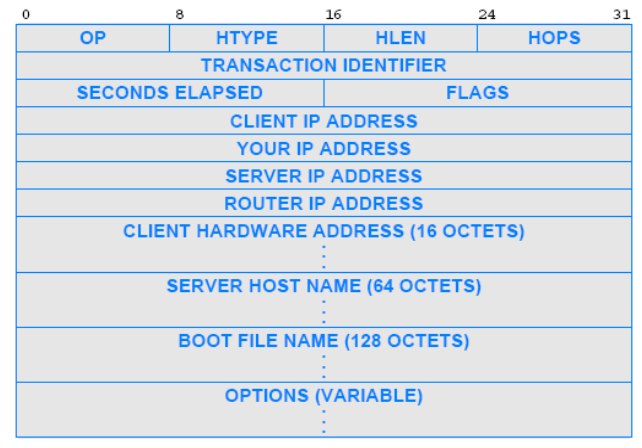
\includegraphics[width=0.5\textwidth]{04/dhcp-message.png}
                \caption{Formato dei messaggi \texttt{DHCP}}
            \end{figure}
            
            Vediamo ora a cosa servono i principali parametri:
            \begin{description}
                \item[\texttt{OP}] Campo di 1 byte che indica se il messaggio è un \textit{request} o un \textit{reply}
                \item[\texttt{HTYPE} e \texttt{HLEN}] Campi di 1 byte l'uno specificano il tipo di \textit{hardware} e la lunghezza dell'indirizzo \texttt{MAC}
                \item[\texttt{FLAGS}] Campo di 2 byte che contiene, ad esempio, se il mittente può ricevere \textit{broadcast} o solo risposte dirette
                \item[\texttt{HOPS}] Campo di 1 byte che indica quanti \textit{server} hanno inoltrato la risposta
                \item[\texttt{TRANSACTION IDENTIFIER}] Campo di 4 byte che identifica la transazione
                \item[\texttt{SECONDS ELAPSED}] Campo di 2 byte che indica da quanto tempo il \textit{client} è in attesa
                \item[\textit{altri}] Ci sono altri campi che indicano l'indirizzo \texttt{IP} del \textit{client}, l'indirizzo \texttt{IP} del \textit{server}, l'indirizzo \texttt{IP} del \textit{router} e l'indirizzo \texttt{IP} del \textit{DNS}.
            \end{description}
        \subsubsection{Se non c'è un \textit{server} \texttt{DHCP}}
            Se non c'è un \textit{server} \texttt{DHCP} allora ci sono due situazioni: la prima è si configura un indirizzo \texttt{IP} statico, mentre, se non riceviamo risposta dopo un certo periodo di tempo, l'\textit{host} provvede all'impostazione di un indirizzo \textit{link-local} che permette la comunicazione con altri \textit{host} nella stessa rete che hanno lo stesso problema.
            \paragraph{Configurazione \textit{link-local}} Per configurare un indirizzo \textit{link-local} si seguono i seguenti passi: \begin{enumerate}
                \item Si sceglie un indirizzo \texttt{IP} compreso tra \texttt{169.254.0.1} e \texttt{169.254.255.254} con maschera di rete \texttt{/16}
                \item Si cerca se esiste una interfaccia di rete con un indirizzo \texttt{IP} \textit{link-local} scelto (tramite \texttt{ARP})
                \item[3.a.] Se esiste un'altra interfaccia con lo stesso indirizzo \texttt{IP} allora si ripete il processo
                \item[3.b.] Altrimenti si configura l'indirizzo \texttt{IP} \textit{link-local}
            \end{enumerate}
    \subsection{Il viaggio di un pacchetto}
        Analizziamo ora il viaggio di un pacchetto da un \textit{host} \texttt{A} ad un \textit{host} \texttt{B} in una rete. assumiamo che \texttt{A} conosca l'indirizzo \texttt{IP} di \texttt{B} e l'indirizzo \texttt{UP} del router \texttt{R} (che è il \textit{default gateway}) (Tramite \texttt{DHCP}), inoltre conosce già l'indirizzo \texttt{MAC} del router \texttt{R} (Tramite \texttt{ARP}).\newline
        Quindi in una rete costituita da \texttt{A}, \texttt{R} e \texttt{B}, con \texttt{R} nel mezzo, il pacchetto viaggia in questo modo: \begin{enumerate}
            \item \texttt{A} crea il datagramma \texttt{IP} con sorgente \texttt{A} e destinazione \texttt{B}
            \item \texttt{A} incapsula il datagramma in un frame di livello 2 con indirizzo \texttt{MAC} di \texttt{R} come destinazione e \texttt{MAC} di \texttt{A} come sorgente
            \item Il frame viene inviato alla rete da \texttt{A} a \texttt{R}\footnote{\label{netSwitch}
                In questo punto possono essere presenti all'interno della rete altri dispositivi di livello 2 come \textit{switch} che inoltrano il pacchetto in base all'indirizzo \texttt{MAC}}
            \item Il frame arriva a \texttt{R} che estrae il datagramma \texttt{IP} e lo passa al livello 3
            \item \texttt{R} controlla la tabella di routing e inoltra il pacchetto a \texttt{B}, per fare ciò incapsula il datagramma in un frame con indirizzo \texttt{MAC} di \texttt{B} come destinazione e \texttt{MAC} di \texttt{R} come sorgente
            \item Il frame viene inviato da \texttt{R} a \texttt{B}\footref{netSwitch}
            \item \texttt{B} estrae il datagramma \texttt{IP} e lo passa al livello 3 per l'elaborazione
        \end{enumerate}
    \subsection{\texttt{IPv6}}
        Il protocollo \texttt{IPv6} è un protocollo nato per ampliare la quantità di indirizzi \texttt{IP} disponibili rispetto quelli di \texttt{IPv4}, successivamente si è voluto standardizzarlo anche in quanto il formato dell'\textit{header} velocizza l'elaborazione dei frammenti, inoltre facilita la gestione della qualità del servizio.\subsubsection{Formato del datagramma \texttt{IPv6}}
            Il formato di un frammento è: \textbf{header} da $40$ byte e la frammentazione è proibita.
            \paragraph{Header} L'\textit{header} di un datagramma \texttt{IPv6} è composto da: \begin{itemize}
                \item \textbf{Flow label} Campo di $20$ bit che permette di identificare un flusso di dati.
                \item \textbf{Priority} Campo di $4$ bit che permette di identificare la priorità del pacchetto.
                \item \textbf{Next header} Campo di $8$ bit che permette di identificare il protocollo di trasporto.
            \end{itemize}
        \subsubsection{Cambiamenti rispetto \texttt{IPv4}}
            In quanto la rete è diventata più affidabile è stato rimosso il \textit{checksum}, vengono rimosse le \textit{options} e il \textit{header} è più corto. Inoltre viene introdotto il protocollo \textit{ICMPv6} con più funzionalità rispetto a \textit{ICMP}.
        \subsubsection{Transizione da \texttt{IPv4} a \texttt{IPv6}}
            La transizione da \texttt{IPv4} a \texttt{IPv6} è molto lenta in quanto richiede un cambiamento di infrastruttura molto grande, per questo si è deciso che se un pacchetto \texttt{IPv6} deve transitare obbligatoriamente per una rete \texttt{IPv4} allora il pacchetto viene incapsulato in un pacchetto \texttt{IPv4} e poi inviato alla rete \texttt{IPv4} e poi riconvertito in un pacchetto \texttt{IPv6} alla destinazione.
        \subsubsection{Indirizzi \texttt{IPv6}}
            La lunghezza non permette notazione \textit{dotted decimal} e quindi si usa la notazione esadecimale: Ogni gruppo di $4$ bit è scritto come una cifra $0,1,\dots,9$ o una lettera: $a,b,\dots,f$. In totale $32$ cifre esadecimali costituiscono un indirizzo \texttt{IPv6}.
            \paragraph{Esempio} Un indirizzo di esempio è \texttt{2a03:2880:f108:0083:face:b00c:0000:25de} che è un indirizzo \texttt{IPv6} valido.
            \paragraph{Raggruppamento} Si possono raggruppare $0$ o omettendoli oppure se è un intero gruppo di $0$ si può omettere tutto il gruppo. Ad esempio l'indirizzo \texttt{2a03:2880:f108:0083:face:b00c:0000:25de} può essere scritto come\texttt{2a03:2880:f108:83:face:b00c:0:25de}. 
        \subsubsection{Indirizzi speciali}
            Gli indirizzi speciali di \texttt{IPv6} sono: \begin{itemize}
                \item \textbf{Unspecified address} Indirizzo $0:0:0:0:0:0:0:0$ che indica che l'indirizzo non è assegnato.
                \item \textbf{Loopback address} Indirizzo $0:0:0:0:0:0:0:1$ che indica l'indirizzo di \textit{loopback}.
                \item \textbf{Link-local address} Indirizzo $fe80::/10$ che indica un indirizzo di \textit{link-local}.
                \item \textbf{Site-local address} Indirizzo $fec0::/10$ che indica un indirizzo di \textit{site-local}.
                \item \textbf{Multicast address} Indirizzo $ff00::/8$ che indica un indirizzo di \textit{multicast}.
            \end{itemize}
        
\end{document}